\documentclass[11pt, a4paper, twoside]{article}   	% use "amsart" instead of "article" for AMSLaTeX format

\usepackage{geometry}                		% See geometry.pdf to learn the layout options. There are lots.
\usepackage{pdfpages}
\usepackage{caption}
\usepackage{minted}
\usepackage[german]{babel}			% this end the next are needed for german umlaute
\usepackage[utf8]{inputenc}
\usepackage{color}
\usepackage{graphicx}
\usepackage{titlesec}
\usepackage{fancyhdr}
\usepackage{lastpage}
\usepackage{hyperref}
% http://www.artofproblemsolving.com/wiki/index.php/LaTeX:Symbols#Operators
% =============================================
% Layout & Colors
% =============================================
\geometry{
   a4paper,
   total={210mm,297mm},
   left=20mm,
   right=20mm,
   top=20mm,
   bottom=30mm
 }	

\definecolor{myred}{rgb}{0.7,0.3,0.4}
\definecolor{mygreen}{rgb}{0,0.6,0}
\definecolor{mygray}{rgb}{0.5,0.5,0.5}
\definecolor{mymauve}{rgb}{0.58,0,0.82}

\setcounter{secnumdepth}{4}


% the default java directory structure and the main packages
\newcommand{\dotNetRoot}{../source/dot-net}
\newcommand{\javaRoot}{../source/java}
\newcommand{\webContent}{\javaRoot/UfoWeb/WebContent}
\newcommand{\imagesRoot}{images}
% the default subsection headers
\newcommand{\ideaSection}{Lösungsidee}
\newcommand{\sourceSection}{Source-Code}
\newcommand{\testSection}{Tests}

% =============================================
% Code Settings
% =============================================
\newenvironment{code}{\captionsetup{type=listing}}{}
\newmintedfile[javaSourceFile]{java}{
	linenos=true, 
	frame=single, 
	breaklines=true, 
	tabsize=2,
	numbersep=5pt,
	xleftmargin=10pt,
	baselinestretch=1,
	fontsize=\footnotesize
}
\newminted[javaSource]{java}{
	breaklines=true, 
	tabsize=2,
	autogobble=true,
	breakautoindent=false
}
\newmintedfile[xmlSourceFile]{xml}{
	linenos=true, 
	frame=single, 
	breaklines=true, 
	tabsize=2,
	numbersep=5pt,
	xleftmargin=10pt,
	baselinestretch=1,
	fontsize=\footnotesize
}
\newmintedfile[propertiesFile]{properties}{
	linenos=true, 
	frame=single, 
	breaklines=true, 
	tabsize=2,
	numbersep=5pt,
	xleftmargin=10pt,
	baselinestretch=1,
	fontsize=\footnotesize
}
\newmintinline[inlineJava]{java}{}
\newmintinline[inlineXml]{xml}{}
% =============================================
% Page Style, Footers & Headers, Title
% =============================================
\title{Übung 3}
\author{Thomas Herzog}

\lhead{Übung 3}
\chead{}
\rhead{
\includegraphics[scale=0.10]{FHO_Logo_Students.jpg}}

\lfoot{S1310307011}
\cfoot{}
\rfoot{ \thepage / \pageref{LastPage} }
\renewcommand{\footrulewidth}{0.4pt}
% =============================================
% D O C U M E N T     C O N T E N T
% =============================================
\pagestyle{fancy}
\begin{document}
\setlength{\headheight}{15mm}
%\includepdf[pages={1-3}]{Swe4xA05-BB.pdf}
{\color{myred}
	\section
		{UFO (Ultimate - Festival - Organizer)}
}
Folgende Dokumentation stellt die Gesamtdokumentation der aufbauenden Übung UFO dar, die im Zuge der Realisierung iterativ über die drei Ausbaustufen hinweg erweitert wird. \\

\subsection{Ausbaustufe 1 (ADO.NET)}
Folgender Teil dokumentiert die erste Ausbaustufe der aufbauenden Übung UFO. In diesem Teil wird die Persistenz Schicht in .NET unter Hilfenahme von ADO.NET implementiert. Aufgrund der Analyse der Gesamtaufgabenstellung wurde entschieden das vorerst nur die Persistenz Schicht an sich, also INSERT, UPDATE, DELETE der einzelnen Entitäten realisiert wird, da die Geschäftslogik erst bei der Realisierung der Administration und des Webzugriffs endgültig feststehen wird. \\\\
Im Zuge der Realisierung des Webzugriffs wird auch der Web-Service implementiert werden müssen, der die Daten der Web Applikation zur Verfügung stellt. Dieser soll die Daten bereits gefiltert und strukturiert zur Verfügung stellen, daher besteht eine gewisse Abhängigkeit zwischen dem Web-Service und der Web Applikation sowie auch der Client Administration.\\\\
Daher werden die Web-Service Implementierung und die Administration die eigentliche Geschäftslogik enthalten, die 
in einer Transaktion abgearbeitet und im wesentlichen aus den logischen Prüfungen gegen die Datenbank bestehen wird sowie der Speicherung und Löschung von Entitäten über die Administration. Die einzelnen Datenabfragen, die benötigt werden können einfach hinzugefügt werden.

\subsubsection{Systemaufbau}
Folgend ist der Systemaufbau der Persistenz Schicht dokumentiert.\\\\
Die folgende Auflistung illustriert die Projektstruktur der Persistenz Schicht:
\begin{enumerate}
	\item\emph{UFO.Server.Data.Api}\\
	 Dieses Projekt enthält die Spezifikation der Persistenz Schicht in Form von 	      Interfaces, abstrakten Klassen, Exceptions und den Entitäten, die wie bei einem ORM-Mapper DB unabhängig sein sollen (sofern möglich).
	 \item\emph{UFO.Server.Data.MySql}\\
	 Dieses Projekt enthält die MySql spezifische Implementierung der Persistenz Schicht.
	 \item\emph{UFO.Server.Test.Data.MySql}\\
	 Dieses Projekt enthält die MySql spezifischen Tests der Persistenz Schicht.
	 \item\emph{UFO.Common.Util}\\
	 Dieses Projekt enthält die Utlities für die UFO Infrastruktur in .NET, die nicht spezifisch einen Systemteil zuzuordnen sind.
	 \item\emph{ufo-data-generator}\\
	 Ein kleines Java Projekt welches eine Java Main Klasse enthält und die benötigen Ressourcen um das Testdatenskript zu erstellen. Hierzu wurde \emph{freemarker} verwendet.
\end{enumerate}
Alle .NET Systemteile werden unter dem Namensraum \emph{UFO.*} zusammengefasst.

\newpage
Die folgende Auflistung illustriert die verwendeten Technologien und Frameworks:
\begin{enumerate}
	\item\emph{MySql}\\
	Es wird eine MySql Datenbank verwendet, die Open-Source ist und eine Integration in .NET besitzt.
	\item\emph{NUNIT}\\
	Als Test-Framework wird NUNIT verwendet, da es mehr Funktionalität mitbringt als das Standard Test-Framework integriert in .NET.
	\item\emph{ADO.NET}\\
	Als Persistenz Provider wird wie gewünnscht ADO.NET und kein ORM Mapper verwendet.
	\item\emph{freemarker}\\
	Template-Engine in Java mit der das Testdaten SQL Skript erstellt wird.
\end{enumerate}

\newpage
\subsubsection{Datenbank}
Es wurde als Datenbank MySql und Moderlierungstool MySql Workbench gewählt, da diese Datenbank erstens Open-Source, zweitens eine gute .NET Integration vorhanden ist sowie drittens bereits Erfahrungen mit dieser Datenbank vorhanden waren.\\\\
Es wurden folgende Skripten generiert die einerseits für die Tests und andererseits für die Generierung der Testdaten genutzt werden. Diese Skripten befinden sich im Projekt \emph{UFO.Server.Data.MySql/Resources}.\\
\begin{enumerate}
	\item\emph{createDatabase.sql}\\
	Ein vollständiges Skript für das Anlegen der Datenbank mit allen Constraints und verwendeten Triggern.
	\item\emph{deleteDatabase.sql}\\
	Ein Skript welches alle Einträge in der Datenbank löscht.
	\item\emph{dropDatabase.sql}\\
	Ein Skript für das Droppen der Datenbank UFO.
	\item\emph{createTestData.sql}\\
	Ein Skript welches die Testdaten generiert.
\end{enumerate}
\ \\
Die Testdaten wurden mit einer Java Applikation mit Hilfe von \emph{Freemarker} erstellt, welches eine Template Engine darstellt. Die Daten werden von \emph{*.csv} Dateien zur Verfügung gestellt und anschließend über eine Java Konsolen Applikation verarbeitet. Diese Applikation liest die Daten ein, verpackt diese in Pojos, generiert dynamische Daten, wie z.B.: die Aufführungen mit den Aufführungszeiten und stellt diese Daten einem Template zur Verfügung.

\newpage
Das folgende ER-Diagramm illustriert das implementierte Datenbank Schema.
\begin{figure}[h]
	\centering
	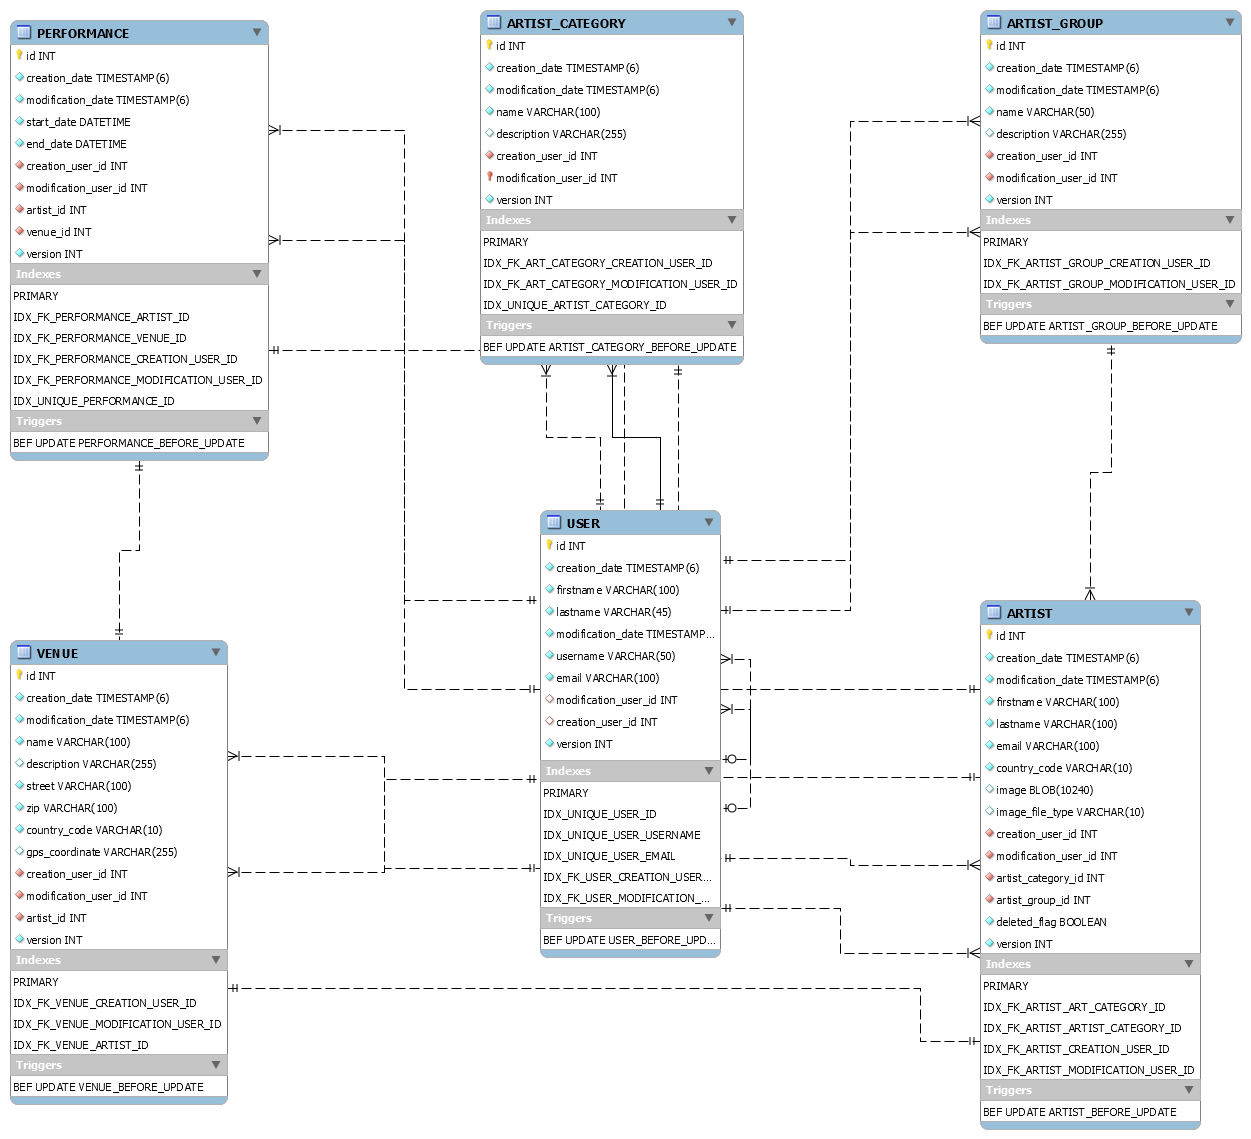
\includegraphics[scale=0.35]{\imagesRoot/er_diagram.PNG}
	\caption
	{ER-Diagramm des Schema 'UFO'}
\end{figure}
\ \\
Auf jeder Entität wurde eine Spalte für die Versionierung eingeführt (MySqlDbType.LONG), die über einen Update-Trigger bei jedem Update um eins erhöht wird sowie auch das Modifizierungsdatum. Ein ganzzahliger Datentyp erschient hier mehr sinnvoll, da es hier mit Sicherheit keine Kollisionen geben kann, nicht so wie bei einem Zeit Datentyp.\\\\
Ebenso halten alle Entitäten eine Referenz auf den Benutzer der Sie erstellt sowie zuletzt modifiziert hat. Dies dient der Nachverfolgbarkeit von Änderungen, zumindest wer zuletzt eine Änderung vorgenommen hat.

\newpage
\subsubsection{Klassenhierarchien}
Folgend sind die Klassenhierarchien der implementierten Klassen und Interfaces dokumentiert.\\

\textbf{\emph{IDao}}\\
Folgendes Klassendiagramm zeigt die Hierarchie des Interfaces \emph{IDao}, das der Basistyp für alle implementierten DAO Interfaces dient, da es bereits alle Basisaktionen auf eine Entität definiert.
\begin{figure}[h]
	\centering
	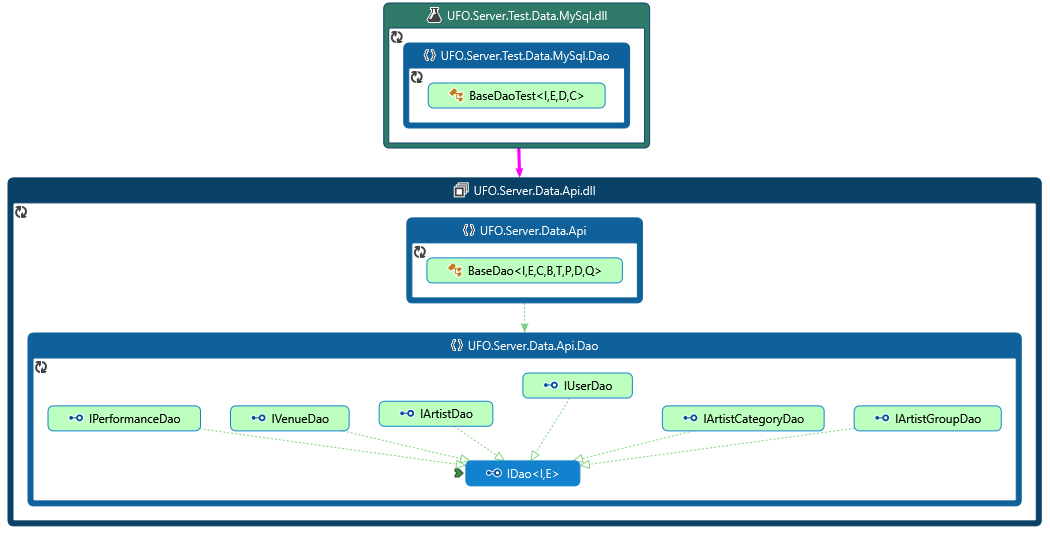
\includegraphics[scale=1]{\imagesRoot/idao_map.PNG}
	\caption
	{Klassenhierarchie IDao Interface}
\end{figure}
\ \\
Die Basisklasse  \emph{BaseDao} implementiert alle Methoden, die in \emph{IDao} definiert wurden für alle implementieren Entitäten sofern sie \emph{IEntity} implementieren. Dieser generische und abstrakte Ansatz erlaubt es dass die Basisfunktionalität eines DAOs nur einmal für alle Entitätstypen, die \emph{IEntity} implementieren, implementiert werden musste.\\\\
Die \emph{DAOs} für die einzelnen Entitäten werden zukünftig Methoden implementieren, die spezifische Datenbankabfragen realisieren, die z.B.: eine komplexe \emph{where caluse} aufweisen, die ihrerseits wieder einen Teil der Geschäftslogik enthält, welche noch nicht vollständig bekannt ist.

\newpage
\textbf{\emph{IEntity}}\\
Folgendes Klassendiagramm illustriert die Klassenhierarchie des Interfaces \emph{IEntity}, welches den Basistyp für alle Entitäten darstellt.
\begin{figure}[h]
	\centering
	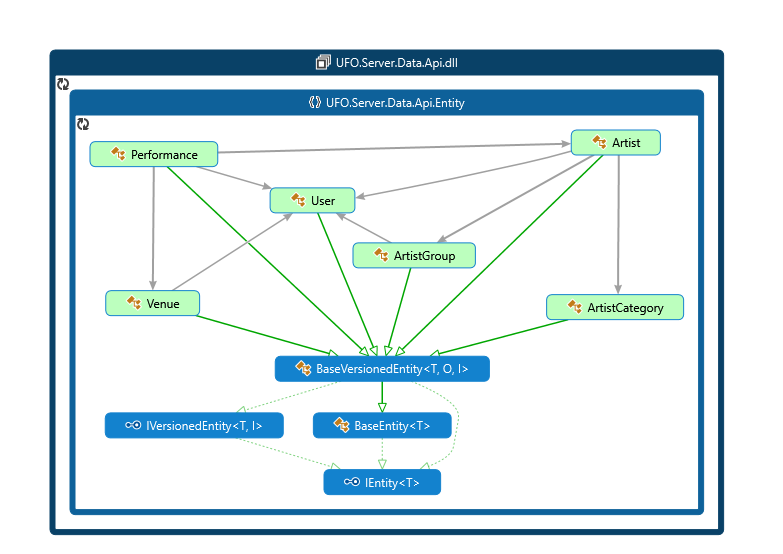
\includegraphics[scale=1]{\imagesRoot/ientity_map.PNG}
	\caption
	{Klassenhierarchie IEntity Interface}
\end{figure}
\ \\
Es wurden Basisentitäten eingeführt, welche eine Basisstruktur definieren dies sich Entitäten unterwerfen müssen wenn sie von diesen Klassen ableiten. Somit wird eine konsistente Struktur der Entitäten bzw. deren Tabellenrepräsentation gewährleistet.\\\\
Die Aufteilung von \emph{IEntity} und \emph{IVersionedEntity} wurde eingeführt, da eine Entität nicht zwangsweise versionierbar sein muss. Ebenso wurde mit den abstrakten Klassen verfahren, die jetzt eine Hierarchie abbilden anstatt die gesamte Funktionalität in eine abstrakte Klasse zu packen.

\newpage 
\textbf{\emph{IEntityHelper}}\\
Folgendes Klassendiagramm illustriert die Klassenhierarchie des Interfaces \emph{IEntityHelper} welches die Utility Methoden für das generieren von Entitäten definiert.
\begin{figure}[h]
	\centering
	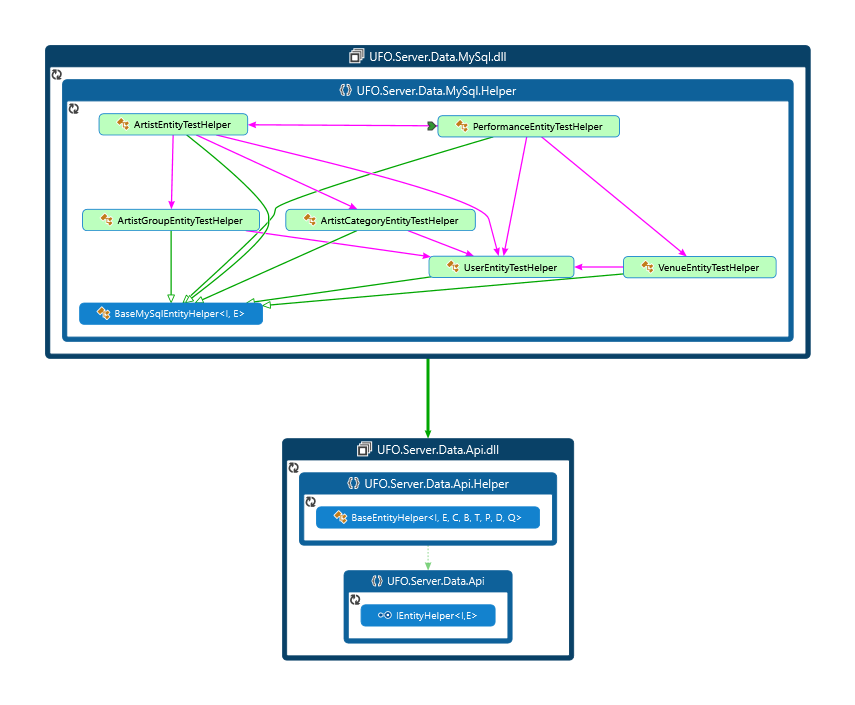
\includegraphics[scale=1]{\imagesRoot/ientityhelper_map.PNG}
	\caption
	{Klassenhierarchie IEntityHelper Interface}
\end{figure}
\ \\
Dieses Interface und dessen Implementierungen diesen als Hilfestellung für die Test und die Generierung von Testdaten über die Entitäten Modelle. Die abstrakte Basisklasse \emph{BaseEntityHelper} implementiert einige der Interface Methoden und stellt eine Persistenzprovider unabhängige Implementierung für das einfache Speichern von Entitäten zur Verfügung. Diese Hilfsklassen entstanden aufgrund der generischen Testklasse \emph{BaseDaoTest}, die die Entitäten nicht erzeugen kann und daher diese von außen zur Verfügung gestellt werden müssen.

\newpage
\textbf{\emph{BaseCommandBuilder}}\\
Folgendes Klassendiagramm illustriert die abstrakte Klasse \emph{BaseCommandBuilder} die das Handling mit einen \emph{DbCommand} beinhaltet. 
\begin{figure}[h]
	\centering
	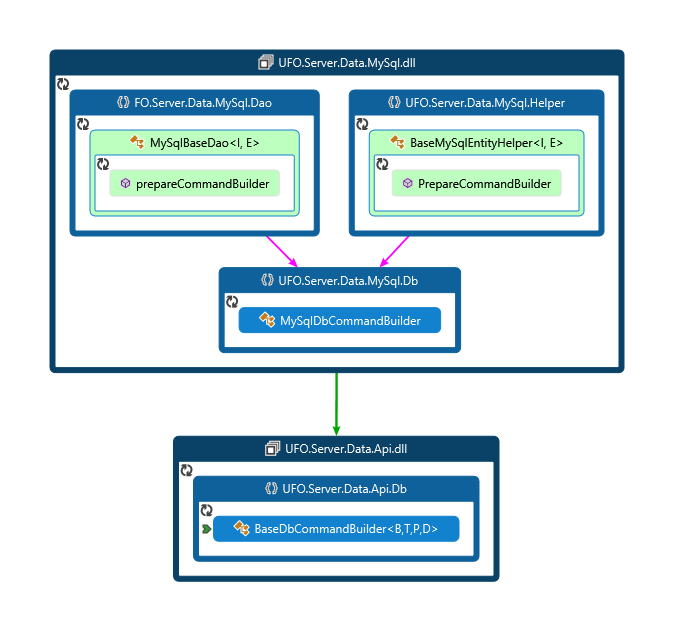
\includegraphics[scale=1]{\imagesRoot/basecommandbuilder_map.PNG}
	\caption
	{Klassenhierarchie der abstrakte Klasse BaseCommandBuilder}
\end{figure}
\ \\
Um zu vermeiden sich mit dem Code des Erstellens, Modifizierens und Verwerfens eines \emph{DbCommand}, in unserem Fall ein \emph{MySqlDbCommand}, herumschlagen zu müssen, wurde beschlossen eine Hilfsklasse einzuführen, die uns dieses Handling mit einem \emph{DbCommand} abnimmt.
Da sich hier eine Fluent-API gut anwenden lässt, wurde diese Funktionalität in Form eines Builder abgebildet.

\newpage
\textbf{\emph{IQueryCreator}}\\
Folgendes Klassendiagramm illustriert das Interface \emph{IQueryCreator}, die die Datenbank spezifischen Statements enthält.
\begin{figure}[h]
	\centering
	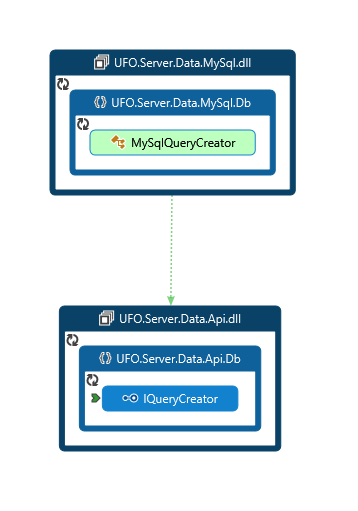
\includegraphics[scale=1]{\imagesRoot/iquerycreator_map.PNG}
	\caption
	{Klassenhierarchie des Interface \emph{IQueryCreator}}
\end{figure}
\ \\
Diese Interface abstrahiert die Datenbank spezifischen Statements von der Klient Logik. Ebenso erlaubt sie es alle Statements in einem Interface abzubilden und diese an einer Stelle pro Entität zu bündeln. 

\newpage
\subsubsection{Hilfsklassen}
Im folgenden werden die Hilfsklassen beschrieben, die eingeführt wurden um sich wiederholende und daher immer wiederkehrende Funktionalitäten zu kapseln und zentral zur Verfügung zu stellen.\\\\

\textbf{\emph{EntityMetamodel}}\\
Diese Klasse löst die Meta-Informationen eines \emph{IEntity} Typs auf und stellt diese aufbereitet nach außen zur Verfügung. Da sich diese Daten zur Laufzeit nicht ändern und daher nur einmalig erzeugt werden sollen, wird eine Factory \emph{EntityMetamodelFactory} eingeführt, die  das Caching der \emph{EntityMetamodel} übernimmt.\\\\

\textbf{\emph{EntityBuilder}}\\
Diese Klasse wurde eingeführt um die Transformation von den Entitäten zur Datenbank und visa versa zu unterstützen, wobei hier einerseits die Werte der Properties, die auf die Datenbank serialisierbar sind, ausgelesen und auf den Property gemapped werden und andererseits die De-Serialisierung vom \emph{IDataReader} zu einer Entität.\\\\

\textbf{\emph{IDbTypeResolver}}\\
Implementierungen dieses Interface lösen einen C\# Typ in einen korrespondierenden Datenbank spezifischen Typ auf.\\\\

\textbf{\emph{DbConnectionFactory}}\\\\
Diese Klasse erstellt und verwaltet die verwendeten \emph{DbConnection} Instanzen. Der Typ der zu verwendenden \emph{DbConnection} wird über die \emph{App.config} definiert, sowie der \emph{ConnectionString}.

\newpage
\subsubsection{Tests}
Die Tests bestehen aus einer einzigen Testklasse, die das \emph{IDao} Interface bzw. die dessen Ableitungen bzw. dessen Implementierungen, die zurzeit nur aus der Implementierung in \emph{BaseDao} bestehen. Also die Basis Dao Funktionalitäten beinhalten wie.\\
\begin{enumerate}
	\item\emph{dao.ById // Throws Exception}
	\item\emph{dao.Find // Returns null}
	\item\emph{dao.Update}
	\item\emph{dao.Persist}
	\item\emph{dao.Delete}
	\item\emph{dao.CheckIfExists}
\end{enumerate}
Die generische Testklasse \emph{BaseDaoTest}  wird mit \emph{NUNIT} Attributen versehen, die die Testklasse mit den zur Verfügung gestellten Typen instanzieren. Danach wird in der Setup Methode die verwendeten Ressourcen über Reflection instanziert und in der Tear-Down Methode disposed. Hier ist die Typinformation zur Laufzeit sehr Hilfreich. In Java als Beispiel würde hier dies Javas Type Erasure unmöglich machen.
\begin{figure}[h]
	\centering
	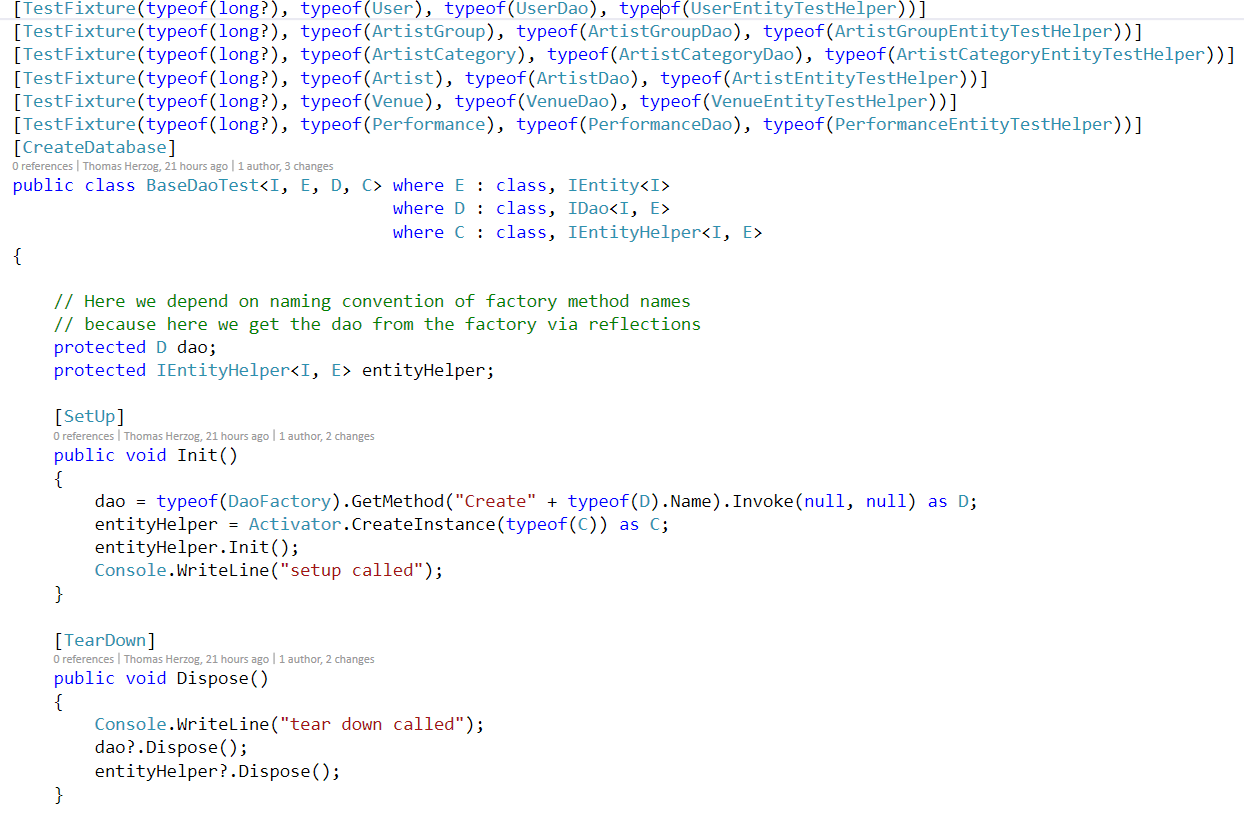
\includegraphics[scale=0.65]{\imagesRoot/basedaotest_screenshot.PNG}
	\caption
	{Ausschnitt aus der Testklasse \emph{BaseDaoTest}}
\end{figure}

\subsection{Ausbaustufe 2 (Commander)}
Folgender Teil dokumentiert die zweite Ausbaustufe des Projektes \emph{UFO} in dem die Administration mit WPF implementiert werden sollte.\\\\
Folgende Projekte wurden der Solution hinzugefügt.
\begin{enumerate}
	\item\emph{UFO.Commander.ServiceApi}\\
	Diese Projekt enthält die Schnittstellen Spezifikation für den Service Layer.
	\item\emph{UFO.Commander.Service.Impl}\\
	Dieses Projekt enthält die Implementierungen der Service Schnittstellen Spezifikationen
	\item\emph{UFO.Commander.Wpf.Administration}\\
	Dieses Projekt enthält die WPF Anwendung, die die Administration abbildet.
\end{enumerate}
\ \\
Des Weiteren wurde der Wurzelnamensraum auf \emph{UFO} beschränkt unter dem jetzt alle Projekte liegen.
\subsubsection{Mögliche Probleme}
Mir ist aufgefallen dass Code im statischen Kontext beim Visual Designer zu Problemen geführt hat, da dieser anscheinend evaluiert wird. Sollten Sie also auf Probleme stoßen so liegt es an folgender Klasse \emph{UFO.Commander.Service.Api.Base.ServiceFactory}.
\newline\newline
Des Weiteren viel mir auf das MySql anscheinend in meiner Version bei einem Prefix diesen nicht in das ResultSet übernimmt. Also eine Query folgendermaßen aussehen könnte.\newline
\emph{SELECT artist.*, venue.* FROM ...} ein Result liefert wie \emph{id, name, id, name}. Sollten Sie eine neuere Version als \emph{5.6.20} könnte dies auf der Performance View Probleme verursachen, da ich davon ausgehe dass diese Verhalten auftritt. 
\subsubsection{Klassenhierarchien}
Folgender Teil der Dokumentation dokumentiert die definierten Klassenhierarchien der WPF Anwendung und des Service Layers.
\newpage
\emph{\textbf{IService}}\\
Folgendes Klassendiagramm zeigt die Hierarchie des Interfaces \emph{IService}, welche die Wurzel aller Service Interfaces darstellt und \emph{IDisposable} erweitert. Somit ist jeder abgeleiteter Service dazu gezwungen die Methode \emph{Dispose} zu implementieren um dort seine gebundenen Ressourcen freizugeben. Des Weiteren wurde eine Basisklasse namens \emph{BaseService} eingeführt, welche die Datenbankverbindung und Transaktionsmethoden implementiert, sodass die abgeleitet Klassen diese Nutzen können.
\begin{figure}[h]
	\centering
	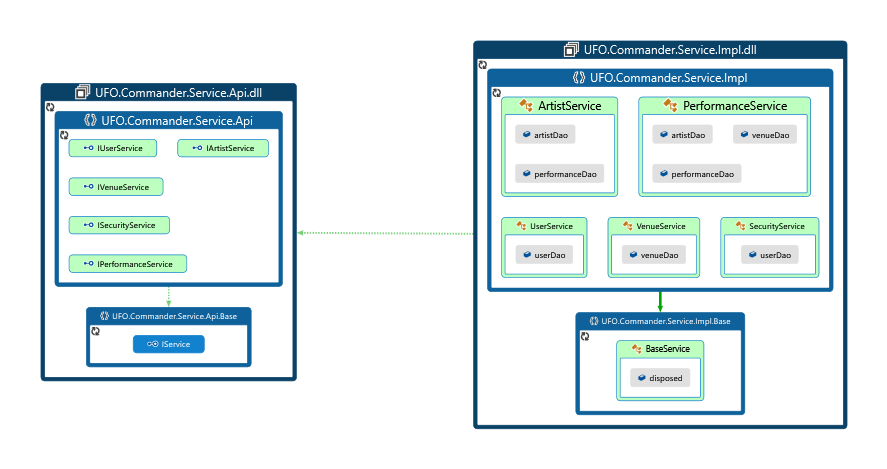
\includegraphics[scale=0.8]{\imagesRoot/iservice_map.PNG}
	\caption
	{Basis Interface für Service Interfaces und Implementierungen}
\end{figure}
\ \\
Alle Services bekommen in Ihrem Konstruktor eine \emph{DbConnection} Instanz übergeben, da alle verwendeten \emph{DAO} Implementierungen dieselbe Datenbank Verbindung nutzen müssen, damit alle sich in derselben Transaktion bewegen.

\newpage
\textbf{\emph{ITabModel}}\\
Folgendes Klassendiagramm zeigt die Hierarchien des Interfaces \emph{ITabModel}, die Operationen definiert, die von der Klasse \emph{TabController} verwendet werden. Die Klasse \emph{TabController} wurde eingeführt um \emph{ITabModel} Instanzen zu initialisieren und beim Wechseln eines Tab aufzuräumen.
\begin{figure}[h]
	\centering
	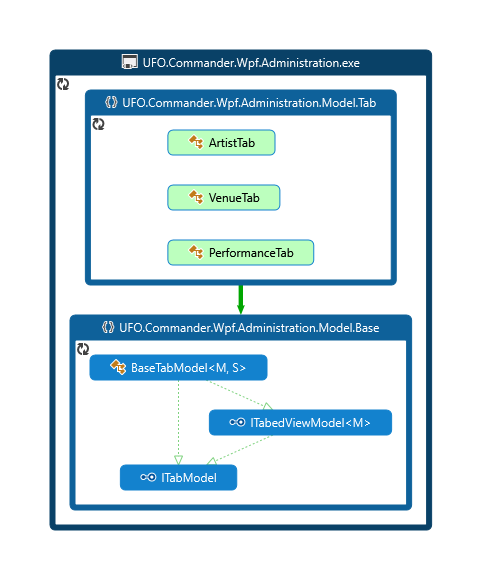
\includegraphics[scale=0.8]{\imagesRoot/basetabmodel_map.PNG}
	\caption
	{Basis Interface für Tab-Model Implementierungen}
\end{figure}
\ \\
Das Interface \emph{ITabedViewModel} definiert die Struktur der Implementierten Tab-Klassen, somit verhält sich jeder Tab gleichermaßen und kann beliebig erweitert werden, je nach seinem View-Content.

\newpage
\textbf{\emph{BasePropertyChangeViewModel}}\\
Folgendes Klassendiagramm zeigt die Hierarchien der Basisklasse \emph{BasePropertyChangeViewModel}, die die Wurzelklasse aller implementierten \emph{View-Models} darstellt, da es immer mindesten einen Property gibt der diesen Event benötigt. Des Weiteren wurde die Klasse \emph{BaseValidationViewModel} eingeführt, die die erste Ableitung von \emph{BasePropertyChangeViewModel} darstellt und die Logik für die Validierung über \emph{System.ComponentModel.DataAnnotations} realisiert. Von dieser Klasse erbt die Basisklasse \emph{BaseEntityViewModel}, die als Wrapper für ViewModels verwendet wird, die eine \emph{IEntity} Instanz für die View wrappen.
\begin{figure}[h]
	\centering
	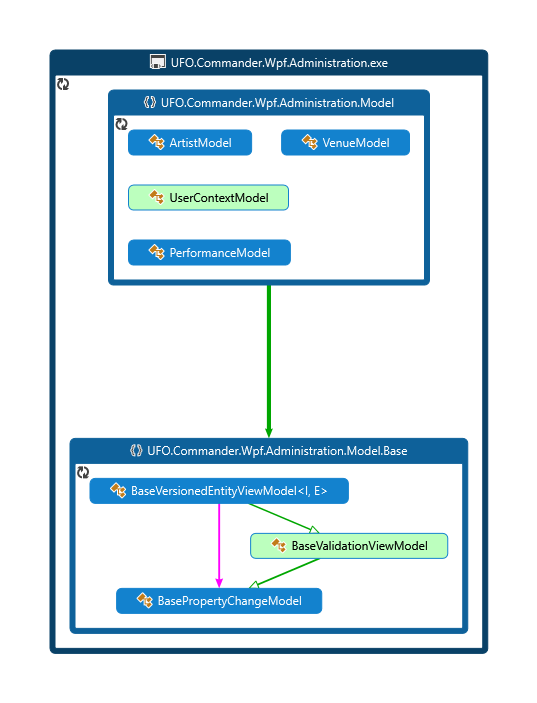
\includegraphics[scale=0.8]{\imagesRoot/viewmodelinheritance_map.PNG}
	\caption
	{Basisklasse für View-Models}
\end{figure}
\ \\
Die Klasse \emph{UserContextModel} wurde eingeführt um einen eingeloggten Benutzer zu repräsentieren und wird als statischer Property der Klasse \emph{App} definiert, da es nur einen eingeloggten Benutzer pro gestarteter Anwendung geben kann. Alle Klassen, die auf den UserContext angewiesen sind müssen die Instanz der Klasse \emph{App} verwenden.

\newpage
\textbf{\emph{SimpleObjectModel}}\\
Folgendes Klassendiagramm zeigt die Hierarchien der Klasse \emph{SimpleObjectModel}, die eingeführt wurde um in Listen, Comboboxen und dergleichen Entitäten für die Darstellung zu halten. Die Controls verwenden Konverter, in denen aus der String Repräsentation wieder in die Entität konvertiert wird. Diese Klasse hält hierbei eine Object Instanz (z.B.: Artist) und den anzuzeigenden Label. In den Konvertern wird eine Instanz \emph{SimpleObjectModel} aus dem zu verwaltenden Objekt erzeugt und visa versa.
\begin{figure}[h]
	\centering
	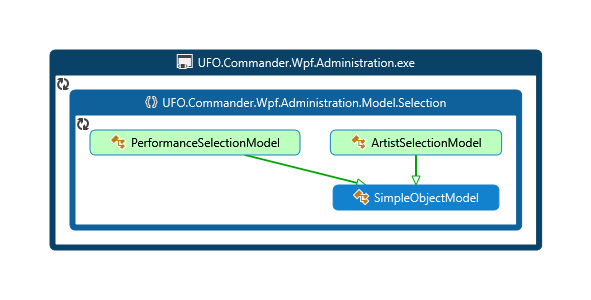
\includegraphics[scale=0.8]{\imagesRoot/simpleobjectmodel_map.PNG}
	\caption
	{Klasse für Controls mit Konverter}
\end{figure}
\ \\
Die beiden abgeleitet Klassen erweitern hierbei die Klasse \emph{SimpleObjectModel} um spezifische Attribute, die in den Controls verwendet werden.

\newpage
\textbf{\emph{IConverter}}\\
Folgendes Klassendiagramm zeigt die Hierarchien der Klasse \emph{IConverter}.
\begin{figure}[h]
	\centering
	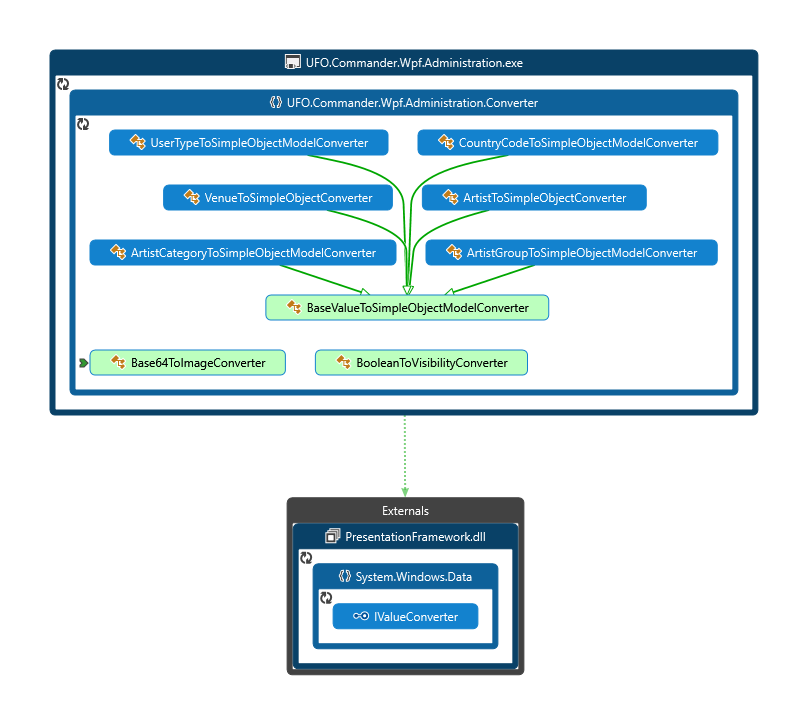
\includegraphics[scale=0.8]{\imagesRoot/iconverter_map.PNG}
	\caption
	{Konverter Hierarchie}
\end{figure}
\ \\
Die Klasse \emph{BaseValueToSimpleObjectConverter} stellt die Basisklasse aller Konverter dar, die Instanzen von \emph{SimpleObjectModel} konvertieren. In diese Klasse wurden alle gemeinsamen Funktionalitäten wie 
\begin{enumerate}
	\item\emph{Typ-Prüfung}\\
	Es wird geprüft ob der Typ des übergebenen Value dem erwarteten Typ entspricht
	\item\emph{ConvertBack}\\
	Da hier nur Instanzen von \emph{SimpleObjectModel} konvertiert werden kann diese Methoden in einer Basisklasse implementiert werden, da hier nur auf den Property \emph{Data} zugegriffen wird.
\end{enumerate}
\ \\
Es wurden auch Konverter für die Visibility (true=Visibility.VISIBILE, false=Visibility.HIDDEN) und zum dekodieren von Base64 Strings in Image Instanzen eingeführt.

\newpage
\subsubsection{WPF Struktur}
Folgende Abbildung zeigt wie die Views innerhalb des Projektes strukturiert wurden.
\begin{figure}[h]
	\centering
	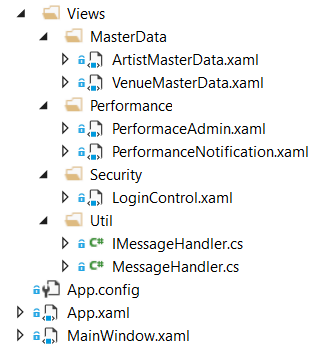
\includegraphics[scale=0.8]{\imagesRoot/viewfolderstructure.PNG}
	\caption
	{Verzeichnisstruktur der Views innerhalb des Projektes}
\end{figure}
\ \\
Bis auf die \emph{App.xaml} und \emph{MainView.xaml} wurden alle Views innerhalb eines Verzeichnis names \emph{Views} gebündelt wobei hierbei eine Trennung zwischen den einzelnen Typen der Views duchgeführt wurde.
\begin{enumerate}
	\item\emph{MasterData}\\
	Alle Views für dier Verwaltung der Stammdaten
	\item\emph{Performance}\\
	Alle Views für die Verwaltung des Festivalprogramms
	\item\emph{Security}\\
	Die Login-View
	\item\emph{Util}\\
	Utility Klassen um innerhalb von View-Models mit der View zu interagieren ohne Referenzen auf WPF Namespaces verwenden zu müssen.
\end{enumerate}
\ \\
Alle diese Views sind als UserControls implementiert worden und werden innerhalb von \emph{MainView.xaml} verwendet (außer PerformanceNotification.xaml), die diese UserControls in einem Tab-Control als DataTemplate für die verschiedene Typen der Tab-Models definiert.
\newline
\newpage
Folgende Abbildung zeigt die eingeführte Verzeichnisstruktur um die WPF-Ressourcen innerhalb diese Projektes zu strukturieren.
\begin{figure}[h]
	\centering
	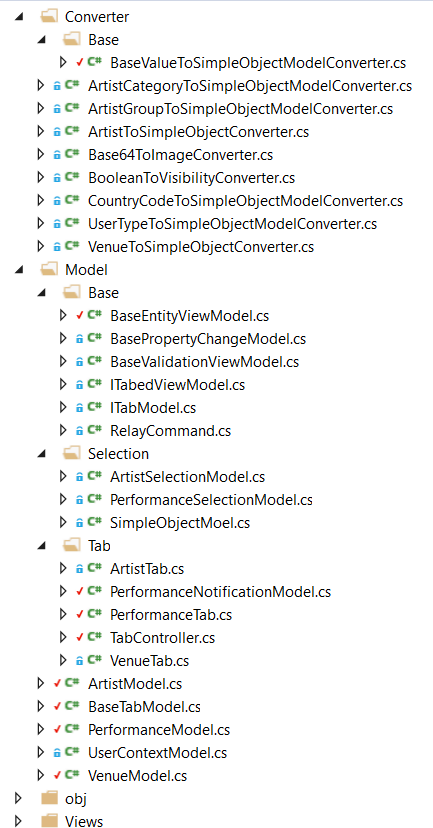
\includegraphics[scale=0.8]{\imagesRoot/wpffolderstrukture.PNG}
	\caption
	{Verzeichnisstruktur der WPF-Ressourcen}
\end{figure}
\ \\
Die jeweiligen Base-Verzeichisse beinhalten die eingeführten Basisklassen für den jeweiligen Kontext (z.B.: Converter, Models, ...).

\newpage
\subsubsection{Benutzerdokumentation}
Folgend ist die Benutzerdokumentation der WPF-Anwendung \emph{Commander} angeführt.
\newline
\newline
\textbf{Login}\newline
Die Administration benötigt einen Login bevor mit Ihr interagiert werden kann. Dazu müssen Sie als Benutzer angelegt worden sein.
\newline
\begin{figure}[h]
	\centering
	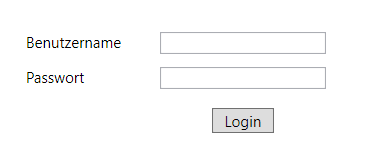
\includegraphics[scale=0.5]{\imagesRoot/view_login.PNG}
	\caption
	{Login nach Start der Anwendung}
\end{figure}
\ \newline
Es wurden keine Beschränkungen beim Login eingeführt, was bedeutet Ihr Zugang wird nach mehrmaligen Fehlversuchen gesperrt.
\newline
\newline
\emph{Mögliche Fehler}
\newline
\newline
Wenn Sie nachdem Start der Anwendung folgende Fehlermeldung erhalten, prüfen Sie bitte ob Sie auf die Datenbank zugreifen können.
\begin{enumerate}
	\item\emph{Fehlende Datenbankverbindung}
	\newline
	Sollten sie keine Datenbankverbindung habe so erhalten Sie folgende Fehlermeldung nach dem Sie die Anwendung gestartet haben. In diesem Fall können Sie sich nicht einloggen.
	\begin{figure}[h]
	\centering
	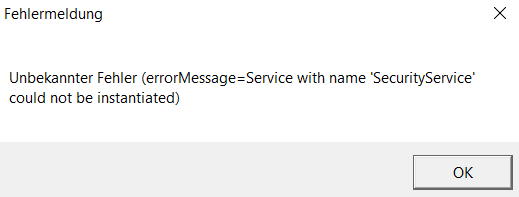
\includegraphics[scale=0.5]{\imagesRoot/view_error_start_app.PNG}
	\caption
	{Fehlermeldung keine Datenbankverbindung}
\end{figure}
\item\emph{Login fehlgeschlagen}
\newline
Wenn Sie ein falsches Passwort eingeben erhalten Sie folgende Fehlermeldung
\begin{figure}[h]
	\centering
	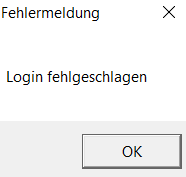
\includegraphics[scale=0.5]{\imagesRoot/view_error_login_failed.PNG}
	\caption
	{Fehlermeldung Login fehlgeschlagen}
\end{figure}
\end{enumerate}
\ \newpage
\parindent0pt{\textbf{Artistenverwaltung}}
\newline
Nachdem Sie sich erfolgreich eingeloggt haben starten Sie mit der Ansicht der Artistenverwaltung, wo Sie die Stammdaten der Artisten verwalten können.
\begin{figure}[h]
	\centering
	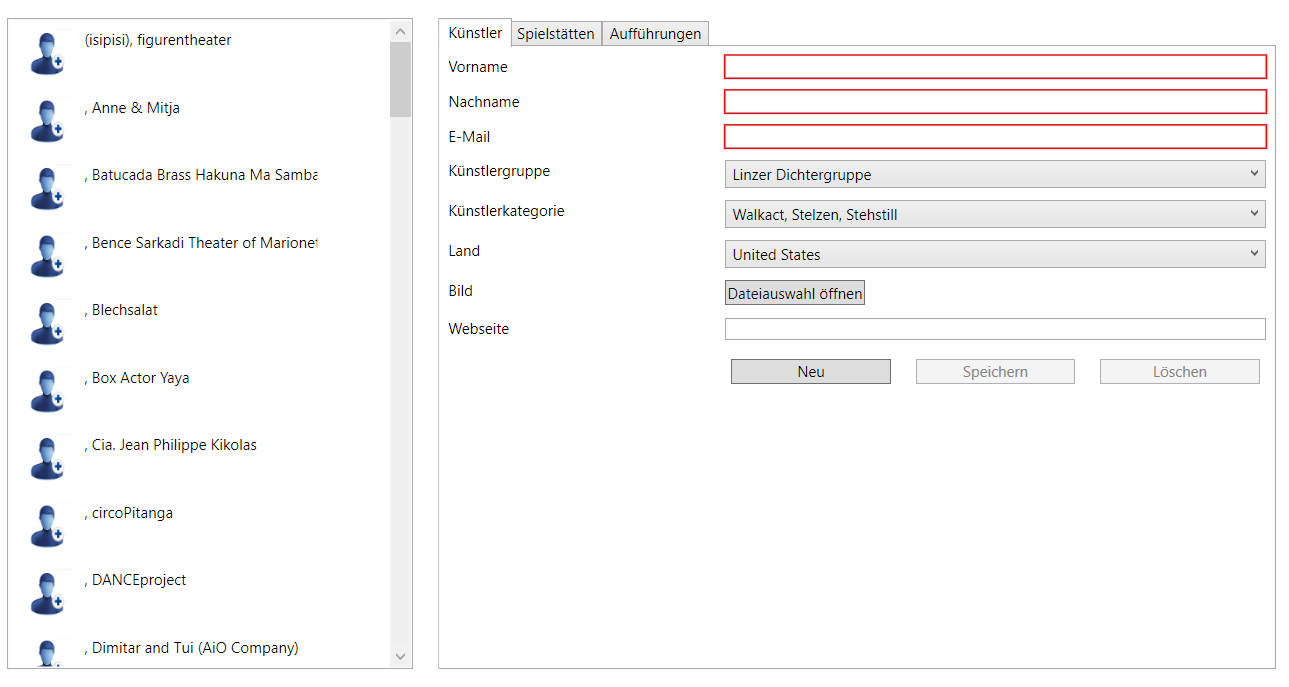
\includegraphics[scale=0.5]{\imagesRoot/view_artist.PNG}
	\caption
	{Stammdatenverwaltung der Artisten}
\end{figure}
\ \newline 
Alle Ansichten sind nachdem selben Schema aufgebaut. Linker Hand sehen Sie die Auswahl der bereits existierenden Einträge - in diesem Fall die Artisten - die Sie auswählen und rechter Hand - innerhalb des Tabs - bearbeiten können. Die rot markierten Eingabefelder signalisieren, dass hier Validierungsfehler aufgetreten sind. Wenn Sie mit dem Cursor über ein rot markiertes Eingabefeld kommen wird Ihnen ein Tooltip angezeigt, der Ihnen mitteilt welcher Validierungsfehler aufgetreten ist.
\newline
\newline
Sollten Sie einen Artisten löschen so werden alle in der Zukunft liegenden Aufführungen dieses Artisten ebenfalls gelöscht. Sollten alle Aufführungen gelöscht worden sein, so wird der Artist ebenfalls gelöscht, andererseits wird der Artist als gelöscht markiert. Auf jeden Fall ist der Artist nicht mehr für Sie verfügbar.
\newline
\newpage
\emph{Mögliche Fehler}
\begin{enumerate}
	\item\emph{Bild zu groß}
	\newline
	Sollten Sie ein Bild auswählen, welches die maximal erlaubte Größe überschreitet, dann erhalten Sie folgende Fehlermeldung
	\begin{figure}[h]
	\centering
	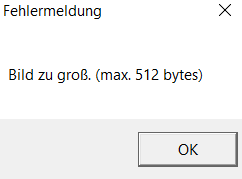
\includegraphics[scale=0.5]{\imagesRoot/view_error_image_too_large.PNG}
	\caption
	{Fehlermeldung Bild zu groß}
\end{figure}
\item\emph{Artist wurde geändert}
\newline
Sollten ein anderer Benutzer den Artisten geändert haben so erhalten Sie folgende Fehlermeldung
	\begin{figure}[h]
	\centering
	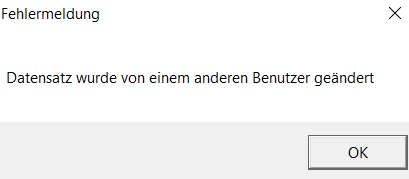
\includegraphics[scale=0.5]{\imagesRoot/view_error_concurrent.PNG}
	\caption
	{Fehlermeldung Artist geändert}
\end{figure}
\item\emph{Artist nicht mehr vorhanden}
\newline
Sollten Sie versuchen einen Artisten zu speichern/löschen und der Artist wurde entweder als gelöscht markiert oder tatsächlich gelöscht, so erhalten Sie folgende Fehlermeldung
	\begin{figure}[h]
	\centering
	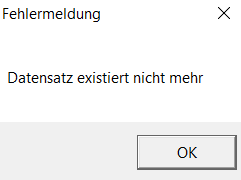
\includegraphics[scale=0.5]{\imagesRoot/view_error_entity_not_existent.PNG}
	\caption
	{Fehlermeldung Artist nicht gefunden}
\end{figure}	
\end{enumerate}
\newpage
\textbf{Spielstätten}
\newline
Auf diesem Tab könne Sie die zur Verfügung stehenden Spielstätten administrieren.
	\begin{figure}[h]
	\centering
	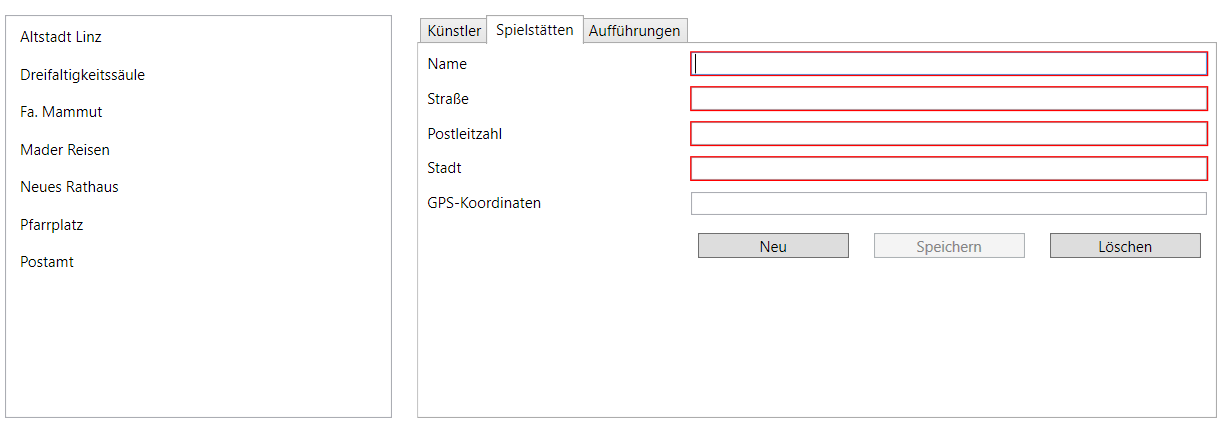
\includegraphics[scale=0.5]{\imagesRoot/view_venue.PNG}
	\caption
	{Stammdatenverwaltung der Spielstätten}
\end{figure}
\ \newline
Bitte stellen Sie sicher das die eingegeben GPS-Koordinaten korrekt sind da hier keine Prüfung auf Korrektheit erfolgt. Sollten Sie GPS-Koordinaten angeben, so können diese in der  Web-Anwendung für Goolge-Maps verwendet werden. Sollten Sie nur die Adressdaten angeben so kann es passieren dass die Position auf Goggle-Maps nicht korrekt angezeigt wird, falls Google diese Adresse nicht kennt oder falsch zuordnet.
\newline
\newline
Sollten bereits Aufführungen an dieser Spielstätte stattfinden, so haben Sie nur mehr die Möglichkeit den Name dieser Spielstätte zu ändern. Bei einem Löschen einer in Verwendung befindlichen Spielstätte wird diese lediglich als gelöscht markiert. In jedem Fall sind gelöschte Spielstätten für Sie nicht mehr verfügbar.
\newline
\newline
\emph{Mögliche Fehler}
\begin{enumerate}
\item\emph{Spielstätte wurde geändert}
\newline
Sollte ein anderer Benutzer die Spielstätte geändert haben so erhalten Sie folgende Fehlermeldung
	\begin{figure}[h]
	\centering
	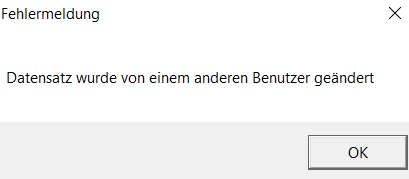
\includegraphics[scale=0.5]{\imagesRoot/view_error_concurrent.PNG}
	\caption
	{Fehlermeldung Spielstätte geändert}
\end{figure}
\item\emph{Spielstätte nicht mehr vorhanden}
\newline
Sollten Sie versuchen eine Spielstätte zu speichern/löschen und die Spielstätte wurde entweder als gelöscht markiert oder tatsächlich gelöscht, so erhalten Sie folgende Fehlermeldung
	\begin{figure}[h]
	\centering
	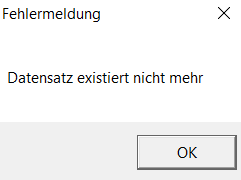
\includegraphics[scale=0.5]{\imagesRoot/view_error_entity_not_existent.PNG}
	\caption
	{Fehlermeldung Spielstätte nicht gefunden}
\end{figure}	
\end{enumerate}
\ \newline
\newpage
\textbf{Aufführungen}
Auf diesem Tab können Sie die Aufführungen verwalten. Diese werden auf die Aufführungstage aufgeteilt und sind in der Auswahl - linker Hand - verfügbar. Hier werden auch Informationen angezeigt wie viele Artisten an wie vielen Spielstätten Aufführungen haben.
	\begin{figure}[h]
	\centering
	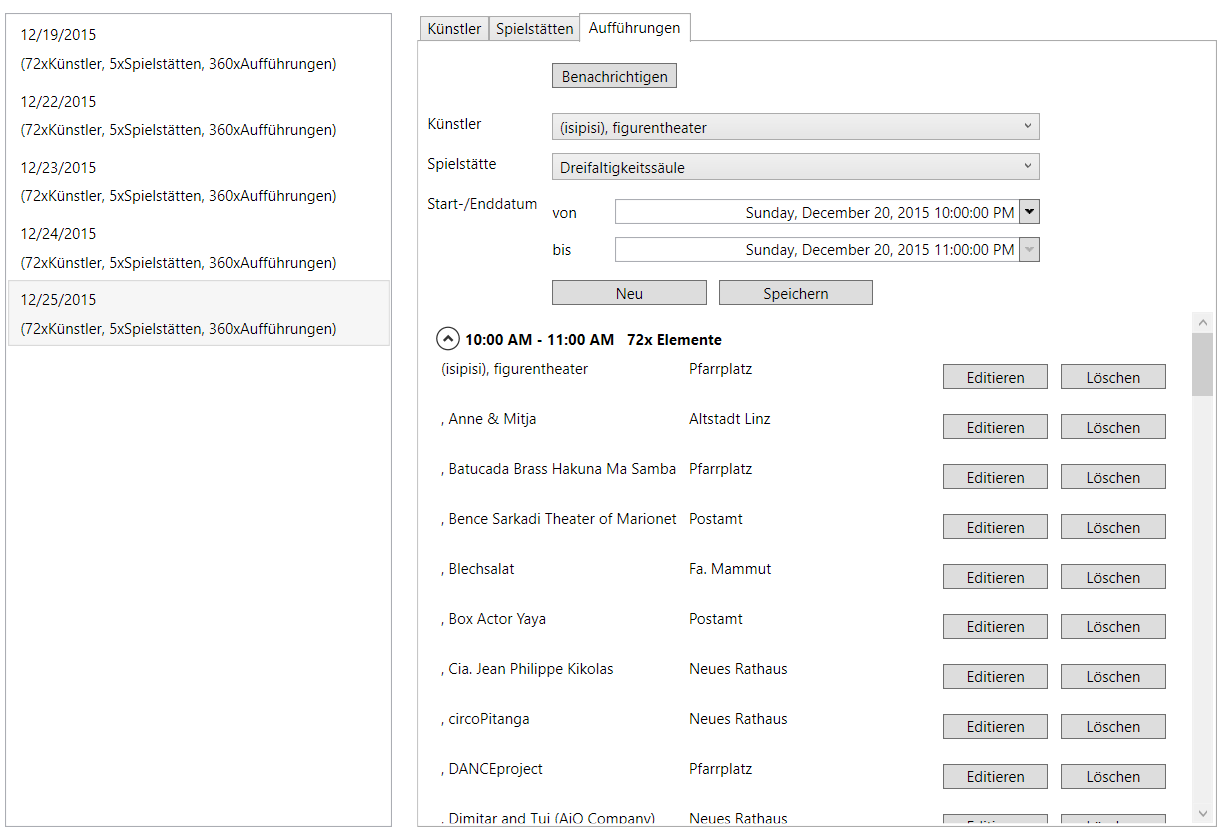
\includegraphics[scale=0.5]{\imagesRoot/view_performance.PNG}
	\caption
	{Festivalverwaltung}
\end{figure}
\ \newline
Nach der Auswahl eines Aufführungstages werden unterhalb des Formulars die Aufführungen geordnet nach der Aufführungszeit, Artistenname und Spielstätte angezeigt. Die Buttons neben den Einträgen signalisieren das diese Einträge änderbar und löschbar sind. Sollten keine Buttons vorhanden sein, so wird diese Aufführung bereits in der Vergangenheit liegen und kann daher weder gelöscht noch geändert werden.
\newline
\newline
Wenn sie auf Editieren klicken so wird das Formular mit den Aufführungsdaten gesetzt und der Button 'Löschen' wird sichtbar. Ansonsten sind die Formularfelder mit Standardwerten befüllt.
\newline
\newline
Wenn Sie den Button 'Benachrichtigen' klicken öffnet sich ein Dialog über den Sie die E-Mail angeben können, die an alle Artisten versendet wird.
	\begin{figure}[h]
	\centering
	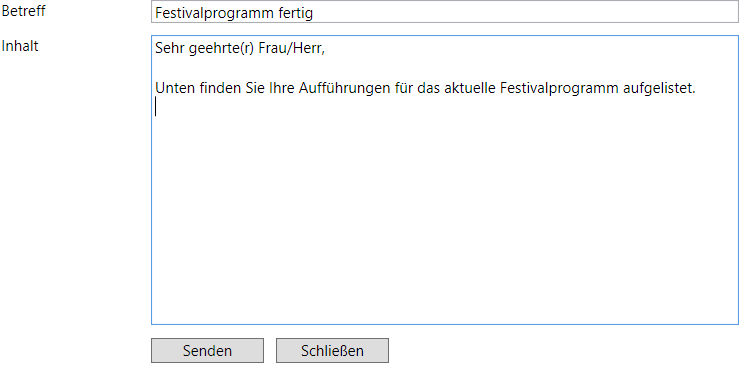
\includegraphics[scale=0.5]{\imagesRoot/view_email_notification.PNG}
	\caption
	{Dialog für E-Mail Benachrichtigungen}
\end{figure}
\ \newline
Diese E-Mail wird an alle Artisten verschickt wobei der E-Mail-Nachricht alle Aufführungen des jeweiligen Artisten angefügt werden.
\newpage
Wenn die E-Mail-Nachrichten versendet wurden erhalten Sie eine Meldung über die Anzahl der versendeten E-Mail-Nachrichten.
	\begin{figure}[h]
	\centering
	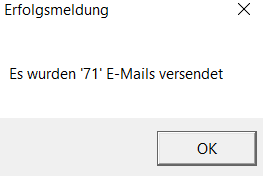
\includegraphics[scale=0.5]{\imagesRoot/view_success_email_sent.PNG}
	\caption
	{Erfolgsmeldung für E-Mail-Versand}
\end{figure}
\ \newline
Sehen Sie hier ein Beispiel für so eine E-Mail Nachricht.
\newline
	\begin{figure}[h]
	\centering
	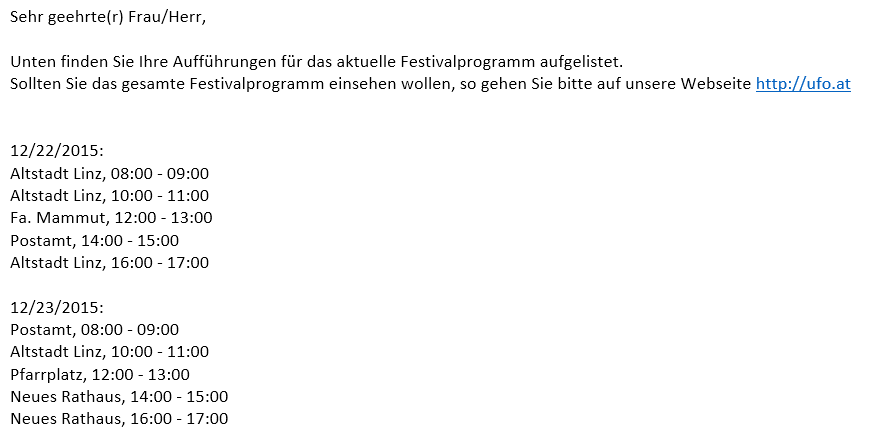
\includegraphics[scale=0.8]{\imagesRoot/sent_email.PNG}
	\caption
	{Generierte E-Mail}
\end{figure}
\ \newline
\newpage
\emph{Mögliche Fehler}
\begin{enumerate}
\item\emph{Aufführung wurde geändert}
\newline
Sollte ein anderer Benutzer die Aufführung geändert haben so erhalten Sie folgende Fehlermeldung
	\begin{figure}[h]
	\centering
	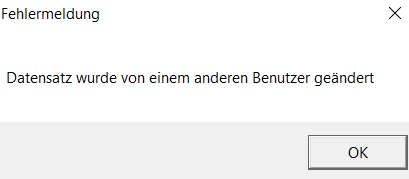
\includegraphics[scale=0.5]{\imagesRoot/view_error_concurrent.PNG}
	\caption
	{Fehlermeldung Spielstätte geändert}
\end{figure}
\item\emph{Aufführung nicht mehr vorhanden}
\newline
Sollten Sie versuchen eine Aufführung zu speichern/löschen und die Aufführung wurde bereits gelöscht so erhalten Sie folgende Fehlermeldung
	\begin{figure}[h]
	\centering
	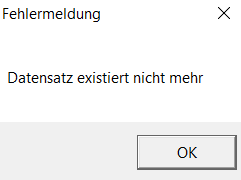
\includegraphics[scale=0.5]{\imagesRoot/view_error_entity_not_existent.PNG}
	\caption
	{Fehlermeldung Spielstätte nicht gefunden}
\end{figure}	
\item\emph{Artist überbucht}
\newline
Sollten Sie versuchen eine Aufführung anzulegen/speichern und der Artist hat bereits eine Aufführung zu diesem Zeitpunkt oder die vordefinierte Pause von 1 Stunde vor und nach einer Aufführung wird unterschritten so erhalten Sie folgende Fehlermeldung
	\begin{figure}[h]
	\centering
	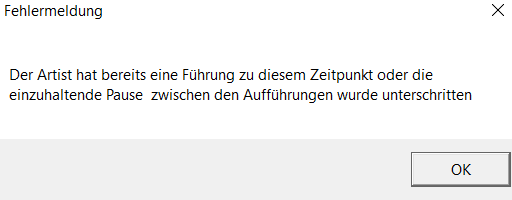
\includegraphics[scale=0.5]{\imagesRoot/view_error_artist_overbooked.PNG}
	\caption
	{Artist überbucht}
\end{figure}
\end{enumerate}
\ \newpage

\subsection{Ausbaustufe 3}
Folgender Teil dieser Dokumentation dokumentiert den dritten Teil der Ausbaustufe. In diesem Teil der Ausbaustufe musste die Web-Anwendung für \emph{UFO} implementiert werden. Dazu wurden folgende Technologien und Frameworks verwendet:
\begin{enumerate}
	\item\emph{Myfaces}
	\newline
	Java-Server-Faces Implementierung von Apache
	\item\emph{Weld}
	\newline
	Context and Dependency Injection Implementierung von Apache
	\item\emph{Deltaspike}
	\newline
	Open-Source CDI-Extension Library, die nützliche Features für eine CDI-Anwendung zur Verfügung stellt.
	\item\emph{Google-Maps-Services}
	\newline
	Google Java-API für Geocoding.
	\item\emph{Jackson-Json}
	\newline
	Open-Source Framework für JSON Mappings
	\item\emph{log4j}
	\newline
	Apache Logging Framework
	\item\emph{Apache-Commons}
	\newline
	Eine Sammlung von common Libraries von Apache wie z.B.: common-collections.
	\item\emph{Primefaces}
	\newline
	Bekannte Open-Source JSF-Komponentenlibary
\end{enumerate}
\ \newline
In dieser Anwendung wurde \emph{CDI} verwendet, damit Abhängigkeiten und Ressourcen über 
Injizierung den Beans zur verfügung gestellt werden konnten. Diese Abhängigkeiten können vom CDI-Container kontextabhängig (verschiedene Scopes) werden. Daher wurde entschlossen CDI in die Anwendung zu integrieren. Dies stellte sich nicht als schwierig heraus, da neben den notwendigen Abhängigkeiten nur geringfügige Konfiguration in der \emph{web.xml} von Nöten war.
\newline
\newline
\emph{Deltaspike} ist eine Erweiterung für CDI und stellt nützliche Features zur Verfügung. Es wurde hierbei das Feature \emph{Type-Safe-Messages} verwendet, dass erlaubt über ein Interface ein \emph{MessageBundle} zu definieren, welches auch über CDI und \emph{EL} verfügbar ist. Hierbei wird über eine CDI-Extension beim Start des Containers dynamisch ein Bean an den Container gebunden, wobei keine explizite Implementierung dieses Beans von Nöten ist.
\newline
\newline
\emph{Google-Maps-Services} wurde dazu verwendet um die Koordinaten der Spielstätten aufzulösen, die keine Koordinaten aber Adressen zur Verfügung stellen. Dadurch können auch diese Spielstätten auf der verwendeten Google-Map angezeigt werden. Die Genauigkeit hängt aber hierbei von den zur Verfügung gestellten Adressdaten ab und natürlich von dem gelieferten Resultat des Geocoding.
\newpage
\subsubsection{Konfiguration}
Die Konfiguration erfolgte hauptsächlich in der \emph{web.xml}. Es wurde vollständig darauf verzichtet die Navigation über die \emph{faces-config.xml} zu implementieren, da einerseits diese Art der Konfiguration mir zu komplex und unflexibel erscheint und andererseits die Anwendung als Single-Page-Anwendung implementiert wurde und daher keine Navigation erforderlich ist.
\newline
\newline
In der \emph{web.xml} wurden alle Konfiguration für die SOAP-Services vorgenommen wie die URLs, die verwendete Zeitzone, den verwendeten Namespace und die Authentifizierungsdaten der Web-Anwendung für die SOAP-Zugriffe. Da es Unterschiede bei der Interpretation der Datumsinformationen in \emph{.NET} (UTC) und \emph{Java} (GMT) gab, musste die Zeitzone konfigurierbar gemacht werden, damit bei der Überfügung von den SOAP-Models in die View-Models die Datumsinformationen mit der richtigen Zeitzone interpretiert werden konnten. Da die Adressen der Services sich ändern könnten wurden diese Adressen ebenfalls in der \emph{web.xml} für jeden Service einzeln konfigurierbar gemacht.  
\begin{code} 
	\caption{web.xml}
	\xmlSourceFile{\webContent/WEB-INF/web.xml}
\end{code}
\ \newpage
Es wurde eine eigene \emph{JsfExceptionHandlerFactory} und eine eigener \emph{JsfExceptionHandler} implementiert sodass die Exceptions nicht mehr an den Client gesendet werden und diese ebenfalls wie gewünscht behandelt werden können. Diese \emph{JsfExceptionHandlerFactory}, die die \emph{JsfExceptionHandler} Instanz erstellt wurde in der \emph{faces-config.xml} registriert.
\begin{code}
	\caption{faces-config.xml}
	\xmlSourceFile{\webContent/WEB-INF/faces-config.xml}
\end{code}
\ \newline
Zusätzlich zu diesen Konfigurationen muss beim Start des Tomcat-Servers JVM-Argumente hinzugefügt werden, damit der Zugriff auf die SOAP-Services über SSL funktioniert.
\newline
\newline
\emph{javax.net.ssl.trustStore}
\newline
\emph{javax.net.ssl.trustStorePassword}
\newline
\newline
Siehe hierzu die Datei \emph{tomcat-config.txt} im Java-Web-Project Root-Verzeichnis. Der Truststore muss natürlich das aktuell von IIS verwendete Zertifikat importieren.
\newpage

\subsubsection{Web-Service-Proxy-Architektur}
Folgende Architektur wurde implementiert um die SOAP-Service Instanzen von der View-Logik zu abstrahieren.
\begin{figure}[h]
	\centering
	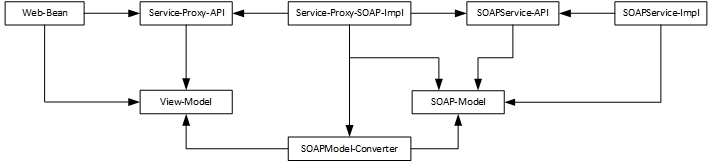
\includegraphics[scale=0.9]{\imagesRoot/service-architecture.JPG}
	\caption
	{Service-Proxy-Architecture}
\end{figure}
\ \newline
Durch diese Architektur wird gewährleistet, dass die Remote-Service Abhängigkeiten vollständig von den View-Beans abstrahiert sind und diese ausgetauscht werden können ohne diese Beans modifizieren zu müssen. Es wurden Konverter eingeführt, die die Remote-Service-Models in die View-Models überführen und nötige Aufbereitungen und Konvertierungen vornehmen. 
\newline
\newline
Die Service-Proxy Instanzen werden über CDI injiziert und wurden als
\newline
\inlineJava{javax.enterprise.context.ApplicationScoped} deklariert, was zur Folge hat das diese Instanzen nur einmalig innerhalb der Anwendungslebenszeit erstellt werden. Dies ist als gleichwertig mit einer Singleton-Instanz anzusehen. Mit den Konvertern wurde gleich verfahren.
\newline
\newline
Im Gegensatz zu den Service-Proxy werden die SOAP-Service-Instanzen über einen Producer erstellt, da hier noch Konfigurationen von Nöten sind und daher die Instanzen nicht von CDI selbst erstellt werden können. Dank \emph{Deltaspike} ist man in der Lage sich den \emph{ServletContext} in CDI-Beans injizieren zu lassen, wobei hier der herkömmliche Ansatz der Konfiguration umgedreht wird. Also nicht ein \emph{ServletContextListener} liest die Init-Parameter aus und konfiguriert ein Bean sondern der Producer liest die Init-Parameter aus und  konfiguriert die zu erstellenden Instanzen. Dies ist ein guter Ansatz da für den Client die Factory im Verborgenen bleibt was der Grundsätzliche Gedanke von \emph{IOC} (Inversion-Of-Control) ist.
\newline
\newline
Die \emph{SOAP-Service} Implementierungen wurden mit dem Standardtool von Eclipse generiert (Apache-Axis), was zwar eine relative alte Implementierung darstellt aber ausreichend für den Anwendungszweck war.
\newline
\newline
Folgende Paketstruktur wurde für die Service-Proxy Ressourcen eingeführt:
\begin{enumerate}
	\item\emph{at.fh.ooe.swk.ufo.service.api}
	\newline
	Enthält die Spezifikation für die Service-Proxy Ressourcen.
	\item\emph{at.fh.ooe.swk.ufo.servce.impl}
	\newline
	Enthält die Implementierung der Service-Proxy-Spezifikation
\end{enumerate}
\newpage

\subsubsection{Web-Application-Resources}
Da es über die gesamte Anwendung hinweg gemeinsam genutzte Ressourcen gibt wurden diese in einem Paket \emph{at.fh.ooe.swk.ufo.web.application.*} zusammengefasst. Hier sind Ressourcen wie folgt gebündelt:
\begin{enumerate}
	\item\emph{at.fh.ooe.swk.ufo.web.application.bean}
	\newline
	Enthält die Beans für den Login, Repräsentation eines eingeloggten BenutzerIn sowie das LanguageBean für die Verwaltung der verwendeten Sprache.
	\item\emph{at.fh.ooe.swk.ufo.web.application.converter}
	\newline
	Enthält die Konverter, die über die über die gesamte Anwendung hinweg genutzt werden können und keine Referenzen auf spezielle Models beinhalten. Z.B.: Konverter für \emph{SelectItem} Instanzen, die als Value Object, Enum Instanzen halten.
	\item\emph{at.fh.ooe.swk.ufo.web.application.model}
	\newline
	Nachdem jedes View-Model eine Entität darstellt und diese auch über eine Id verfügen wurde ein Interface namens \inlineJava{IdHolder<T>} eingeführt, sowie eine abstrakte Klasse
	\newline \inlineJava{AbstractIdHolderModel<T> implements IdHolder<T>}, die dieses Interface und die Methoden \emph{hash}, \emph{equals} sowie Getter und Setter für die Id implementiert.
	\item\emph{at.fh.ooe.swk.ufo.web.application.constants}
	\newline
	Alle definierten Kontextparameter wurden als Enumeration abgebildet. Somit sind diese Parameter nur an zwei Stellen definiert. Einmal in der \emph{web.xml} und ein zweites Mal in der Enumeration.
	\item\emph{at.fh.ooe.swk.ufo.web.application.exceptions}
	\newline
	Enthält die implementierte \emph{JsfExceptionHandlerFactory} und den implementierten \emph{JsfExceptionHandler} für das Behandeln unbehandelter Exceptions. Dadurch wird das rendern der Exceptions zum Client unterdrückt.
	\item\emph{at.fh.ooe.swk.ufo.web.application.listener}
	\newline
	Enthält den \emph{ServletContextListener}, der die \emph{Default Locale} der VM auf die definierte \emph{Locale} in der \emph{web.xml} setzt
	\item\emph{at.fh.ooe.swk.ufo..web.application.message}
	\newline
	Enthält die Deltaspike \emph{MessageBundle} Interfaces und dazugehörigen \emph{RessourceBundles}. Dadurch wird Multilingualität von der Anwendung unterstützt.
	\item\emph{at.fh.ooe.swk.ufo.web.application.producer}
	\newline
	Enthält die Producer, die gemeinsam genutzte Ressourcen kontextabhängig produzieren.
\end{enumerate}  
\ \newline
Es wurde ein JSF-Template implementiert, welches das Layout und die gemeinsam genutzten View-Ressourcen definiert wie: Loading-Dialog und Message-Komponenten. Diese Ressourcen wurden in das Verzeichnis \emph{WEB-INF/templates} gelegt, da diese nicht von außen verfügbar sein sollen und alle Ressourcen in \emph{WEB-INF} implizit von einem Zugriff geschützt sind.
\ \newpage

\subsubsection{Performances-Resources}
Die gesamten Ressourcen der Performance Ansichten wurden in einem Paket mit folgender Struktur gebündelt.
\begin{enumerate}
	\item\emph{at.fh.ooe.swk.ufo.web.performance.constants}
	\newline
	Enthält die Konstanten für die bereitgestellten Suchoptionen, die in Form von Enumerationen abgebildet wurden.
	\item\emph{at.fh.ooe.swk.ufo.web.performance.model}
	\newline
	Enthält alle \emph{View-Models} sowie \emph{Edit-View-Models}, die in den Performance Ansichten verwendet werden.
	\item\emph{at.fh.ooe.swk.ufo.web.performance.page}
	\newline
	Enthält alle \emph{Backing-Beans} für die einzelnen Ansichten, die deren Verhalten steuern bzw, die zur Verfügung gestellten Aktionen bereitstellen. Somit ist \emph{Interaktionslogik} von der \emph{Präsentationslogik} vollständig getrennt.
	\item\emph{at.fh.ooe.swk.ufo.web.performance.support}
	\newline
	Enthält das \emph{Support-Bean}, in dem die gesamte Ladelogik implementiert ist, sowie die Producer Methoden, die die Performance spezifischen Ressourcen bereitstellt. Dadurch werden die \emph{Backing-Beans} von der Ladelogik befreit.	
\end{enumerate}	
\ \newline
Die einzelnen Teile der Ansichten wurden in eigenen \emph{*.xhtml} Dateien implementiert, die im den Verzeichnis \emph{WEB-INF/page} gehalten werden. Lediglich die \emph{index.xhtml}, die die Komposition der Anwendung darstellt, wurde im Root-Verzeichnis platziert und somit die einzige Möglichkeit des Zugriffs auf die Anwendung. Wiederverwendbare Teile wurden wiederum als Kompositionen definiert wie z.B.: die Tooltip Informationen, die an mehreren Stellen verwendet werden.
\newpage

\subsubsection{Multilingualität}
Die gesamte Anwendung unterstützt Multilingualität, obwohl anzumerken ist, dass nur eine Sprache implementiert wurde. Nicht desto trotz können andere Sprachen implementiert werden. Es wurde hierbei der Mechanismus \emph{Type-Safe-Messages} von \emph{Deltaspike} verwendet, welche eine CDI Extension darstellt. Im folgenden ist ein Ausschnitt des Interfaces \inlineJava{MessagesBundle.java} angeführt. 
\begin{listing}[H]    
\caption{MessageBundle.java}    
\begin{minted}{java}
@MessageBundle
@Named("msg")
public interface MessagesBundle extends Serializable {

	@MessageTemplate("{UFO_PROGRAM}")
	String getUfoProgram();
}
\end{minted}
\end{listing}
\ \newline
Folgende Auflistung beschreibt die verwendeten Annotationen im Interface, die dazu verwendet werden um das MessageBundle zu konfigurieren.
\begin{enumerate}
	\item\emph{\inlineJava{@MessageBundle}}
	\newline
	Annotation, die der Deltaspike-CDI-Extension mitteilt, dass es sich hierbei um eine MessageBundle handelt.
	\item\emph{\inlineJava{@ApplicationScoped}}
	\newline
	CDI-Scope-Annotation, die Deltaspike mitteilt eine Bean zu erstellen, welches nur einmalig über die Anwendungslebenszeit existiert.
	\item\emph{\inlineJava{@Named("msg")}}
	\newline
	CDI-Annotation, die dieses Bean über \emph{Expression-Language} zur Verfügung stellt. Wird von der Deltaspike-CDI-Extension bei der Bean-Erstellung berücksichtigt.
	\item\emph{\inlineJava{@MessageTemplate}}
	\newline
	Deltaspike spezifische Annotation, die den Key in der RessourceBundle Datei darstellt.
\end{enumerate} 
\ \newline
Die enthaltenen Getter-Methoden müssen der Java-Bean-Convention folgen damit diese in EL-Expressions verwendet werden können. Um andere Sprachen zu unterstützen müssen jetzt lediglich nur noch die ResourceBundle Dateien für die einzelnen Sprachen angelegt werden. Des weiteren sollte vielleicht ein eigener \inlineJava{org.apache.deltaspike.core.api.message.LocaleResolver} implementiert werden, der die Locale vielleicht aus dem FacesContext auflöst. Es wird in dem oben angeführten Beispiel der bereits mitgelieferte \inlineJava{org.apache.deltaspike.core.impl.message.DefaultLocaleResolver} verwendet, der die VM-Default-Locale verwendet.
\newline
\newline
Folgendes Beispiel zeigt die Verwendung des Interfaces \inlineJava{MessagesBundle.java} in \emph{*.xhtml}.
\begin{listing}[H]    
\caption{MessageBundle Verwendung in *.xhmtl Dateien}   
\begin{minted}{xml}
<h:outputText value="#{msg.firstName}" style="font-weight: bold;" />
\end{minted}
\end{listing}
\ \newpage

\subsubsection{Security}
Die SOAP-Webservices sind über SSL verfügbar, daher musste dem Tomcat-Server eine Truststore-Datei zur Verfügung gestellt werden, die das trusted Zertifikat des SOAP-Servers enthält. Es wurde hierbei in VisualStudio eingestellt, dass die SOAP-Services SSL unterstützen. Sie sind auch noch über HTTP verfügbar, dies sollte aber bei einem Release unterbunden werden. Ebenfalls ist die Web-Anwendung nur über SSL erreichbar, was durch eine Konfiguration in der Tomcat \emph{server.xml} und in der \emph{web.xml} erreicht wurde.
\begin{listing}[H]    
\caption{server.xml}    
\begin{minted}{xml}
	<Connector  SSLEnabled="true" 
			clientAuth="false" 
			keyAlias="ufo"
			keystoreFile="conf/keystore.jks" 
			keystorePass="ufo" 
			keystoreType="jks"
			maxThreads="150" 
			port="8443" 
			protocol="org.apache.coyote.http11.Http11NioProtocol"
			scheme="https" 
			secure="true" 
			sslProtocol="TLS" />
\end{minted}
\end{listing}

\begin{listing}[H]    
\caption{web.xml}    
\begin{minted}{xml}
	<!-- Allow SSL only -->
	<security-constraint>
		<web-resource-collection>
			<web-resource-name>Protected Context</web-resource-name>
			<url-pattern>/*</url-pattern>
		</web-resource-collection>
		<!-- auth-constraint goes here if you requre authentication -->
		<user-data-constraint>
			<transport-guarantee>CONFIDENTIAL</transport-guarantee>
		</user-data-constraint>
	</security-constraint>
\end{minted}
\end{listing}
\ \newline
Des weiteren sind die SOAP-Services nicht offen verfügbar sondern die einzelnen Anwendung müssen registriert sein, ansonsten liefert der Webservice kein Daten zurück. Man kann darüber streiten ob die Daten offen Verfügbar sein sollen, aber in dieser Anwendung sind sie es nicht. Die Zugangsdaten für die Web-Anwendung sind in der \emph{web.xml} definiert und auf der .NET Seite in der \emph{web.config}, wobei hier angemerkt sei, dass dieser Ansatz nur für dieses Beispiel Anwendung finden sollte. Mann sollte hierbei in der Lage sein die Zugangsdaten der Anwendung dynamisch zum Beispiel aus einer Datenbank zu ziehen und sie nicht statisch in einer Konfigurationsdatei halten. Bei einem Deployment einer Web-Anwendung könnte für diese die Zugangsdaten erstellt und in einer Datenbank gespeichert werden.
\newpage
\begin{listing}
\caption{Auszug aus SoapWebServiceProducer.java}
\begin{minted}{java}
@ApplicationScoped
public class SoapWebServiceProducer implements Serializable {

	@Inject
	@DeltaSpike
	private ServletContext servletContext;

	private String username;
	private String password;

	@PostConstruct
	public void postContruct() {
		// Get authentication data from web.xml
		username = servletContext.getInitParameter(
			ContextParameter.WEBSERVICE_USERNAME.key);
		password = servletContext.getInitParameter(
			ContextParameter.WEBSERVICE_PASSWORD.key);
		...
	}
	
	...
	
	private SOAPHeaderElement createSoapHeader() throws Exception {
		SOAPHeaderElement authentication = new SOAPHeaderElement(
				xmlNamespace,
				"Credentials");
		SOAPElement node = authentication.addChildElement("Username");
		node.addTextNode(username);
		SOAPElement node2 = authentication.addChildElement("Password");
		node2.addTextNode(password);

		return authentication;
	}
}
\end{minted}
\end{listing} 
\ \newline
Die Authentifizierungsdaten für die Web-Anwendung werden hierbei über einen SOAP-Header an die Soap-Services übermittelt, die diesen Header auswerten und überprüfen ob es sich um eine registrierten Anwendung handelt.
\newpage
\begin{code}
	\caption{BaseSecureWebservice.cs}
	\javaSourceFile{\dotNetRoot/UFO/UFO.Server.Webservice/Soap/Base/BaseSecureWebservice.cs}
\end{code}
\ \newpage
\begin{listing}
\caption{Auszug auf PerformanceWebservice.cs}
\begin{minted}{java}
	[WebMethod]
        [ScriptMethod(UseHttpGet = false)]
        [SoapHeader("credentials")]
        public ListResultModel<PerformanceModel> GetPerformances(
        	PerformanceFilterRequest filter)
        {
            IPerformanceDao performanceDao = DaoFactory.CreatePerformanceDao();
            ListResultModel<PerformanceModel> model = null;
            if ((model = HandleAuthentication<ListResultModel<PerformanceModel>>()) 
            	== null)
            {
            	...
            }
            ...
        }
\end{minted}
\end{listing}
\ \newline
\inlineJava{BaseSecureWebservice.cs} beinhaltet den Property, der das SOAP-Header-Model darstellt, sowie die Authentifizierungsmethode, die auch das Resultat im Falle einer  fehlgeschlagenen Authentifizierung aufbereitet. Der konkrete Webservice erbt von dieser Klasse und stellt die Daten nur im Falle einer gültigen Authentifizierung zur Verfügung. 
\newline
\newline
Der SOAP-Header wird hierbei vom ASP.NET Framwork über das Attribute \inlineJava{[SoapHeader("credentials")]} in den korrespondierenden Property mit dem definierten Namen injiziert.
\newpage

\subsubsection{SOAP-Services}
Die ASP.NET Soap-Services resultieren immer eine Instanz von \inlineJava{BaseModel.cs}, von der wiederum zwei Klassen ableiten \inlineJava{SingelResultMode.cs} und \inlineJava{ListResultModel.cs}, die jeweils ein Single oder List Resultat halten. Die Basisklasse hält etwaige Informationen über einen Fehler, der in der Web-Anwendung ausgewertet werden könnte. Dadurch sind die Anwendungen, die die Daten abrufen, in der Lage etwaige Fehler korrekt auszuwerten und darauf zu reagieren, da die Fehlerinformationen mit übermittelt werden, wobei aber der Stacktrace ausgeschlossen wurde und nur die Message der Exception übermittelt wird.
\begin{figure}[h]
	\centering
	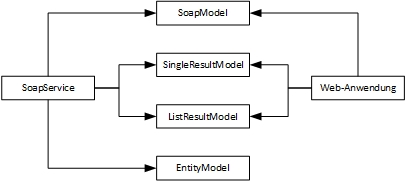
\includegraphics[scale=0.9]{\imagesRoot/soap-model-references.JPG}
	\caption
	{SOAP-Model-Referenzen}
\end{figure}
\ \newline
Wie in der Grafik ersichtlich gibt es keine Referenzen zwischen den Entity-Models und der Web-Anwendung. Es werden alle DAO-Resultate in die entsprechenden SOAP-Models überführt. Somit ist die SOAP-Zugriffsschicht entkoppelt von der Datenbankzugriffsschicht und Änderungen am Datenmodell wirken sich nicht direkt auf die SOAP-Zugriffsschicht aus. Lediglich das Mapping zwischen den Models muss angepasst werden.
\newline
\newline
Es wird sich auf die implizite Konvertierung, die von ASP.NET bereitgestellt wird verlassen, jedoch wurden auch einige XML-Attribute verwendet, wenn z.B.:SOAP-Model-Properties als nullable markiert bzw. dessen XML-Repräsentation definiert werden musste. 
\newpage
\subsubsection{Web-View}
Im folgenden wird der Aufbau der Web-View beschrieben. Die Web-View besteht zwar aus mehreren Templates ist jedoch als Single-Page implementiert. Die einzelnen Teile der Seite sind über ein Layout von einander getrennt. Diese Teile lassen sich ein und ausklappen.
\begin{figure}[h]
	\centering
	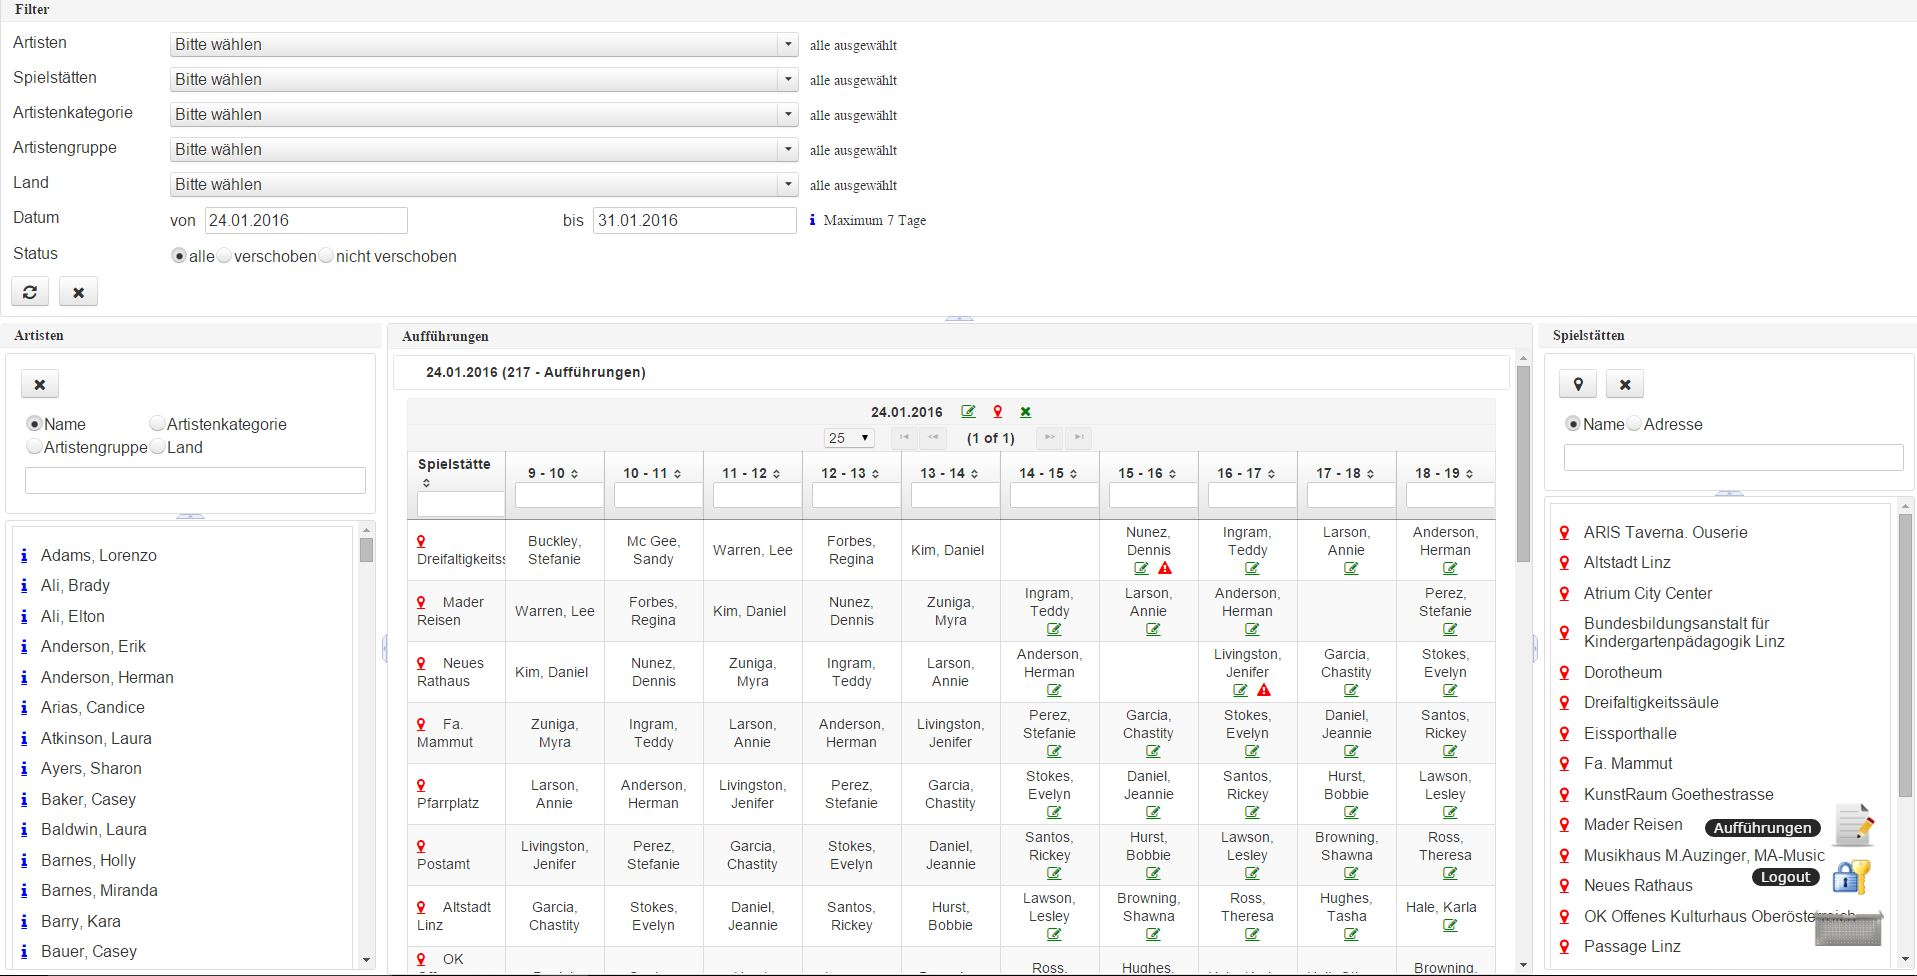
\includegraphics[angle=90, scale=0.36]{\imagesRoot/web-view-full.JPG}
	\caption
	{Vollständige View mit allen Layout-Parts aufgeklappt}
\end{figure}
\ \newpage
Natürlich ist nicht ratsam alle Teile auf zu klappen sondern nur die Teile, die die Informationen bereitstellen, die man benötigt. Lediglich der Center-Content lässt sich nicht weg klappen. Dieser enthält die Tabelle mit allen Aufführungen. Im folgenden werden die einzelnen Teile der Webseite beschrieben.

\paragraph{Filter}
\ \newline
Die folgende Abbildung zeigt die globalen Filter, die die Aufführungsdaten global filtern. Die Daten werden hierbei vom SOAP-Service mit den gesetzten Filtern erneut geladen.
\begin{figure}[h]
	\centering
	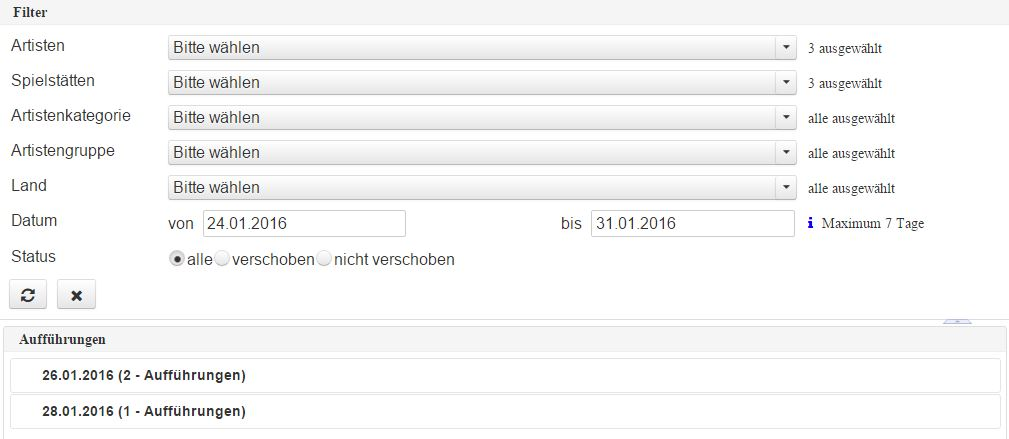
\includegraphics[scale=0.6]{\imagesRoot/web-view-filter.JPG}
	\caption
	{Globale Filter}
\end{figure}
\ \newline
Es stehen hierbei mehrere Filteroptionen zur Verfügung, die alle auf die zu ladenden Daten angewendet werden. Rechts von den Filtern ist die Anzahl der gewählten Optionen angeführt, wobei angemerkt sei, dass wenn keine Optionen ausgewählt wurde es denselben Effekt hat, als währen alle Einträge ausgewählt worden. Der Datumsbereich wurde auf sieben Tage beschränkt. Das Spektakel finden zwar nur an einem Tag statt, jedoch steht es den Entwicklern offen es auch gegebenenfalls für mehrere Tage konfigurieren. Die AnwenderInnen sollten jedoch trotzdem in der Auswahl der Tage eingeschränkt sein, da es einerseits die Performance negativ beeinflussen würde und andererseits es der Übersicht nicht dienlich ist, sich alle tage in einem Jahr anzeigen zu lassen.
\newpage

\paragraph{Artisten}
\ \newline
Dieser Teil der Anwendung zeigt alle verfügbaren Artisten an, die aktiv sind. Es wird hierbei keine Vorfilterung vorgenommen. Auch hier stehen mehrere Option für die Filterung zur Verfügung.
\begin{figure}[h]
	\centering
	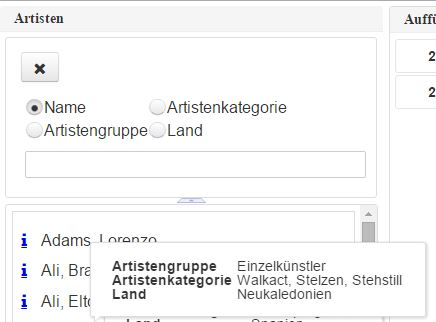
\includegraphics[scale=0.6]{\imagesRoot/web-view-artists.JPG}
	\caption
	{Übersicht Artisten}
\end{figure}
\ \newline
Die Filterung kann entweder nach dem Namen, Artistengruppe, Artistenkategory und des Landes des Artisten erfolgen. Über einen Tooltip werden die wichtigsten Details des Artisten angezeigt. Über den Info-Icon kann ein Dialog geöffnet werden, der alle Details eines Artisten anzeigt. Der Button setzt den gesetzten Filter auf die Standardeinstellungen zurück.

\paragraph{Übersicht Spielstätten}
\ \newline 
Dieser Teil der Anwendung zeigt alle verfügbaren Spielstätten an. Es wird hierbei keine Vorfilterung vorgenommen. Auch hier stehen mehrere Option für die Filterung zur Verfügung.
\begin{figure}[h]
	\centering
	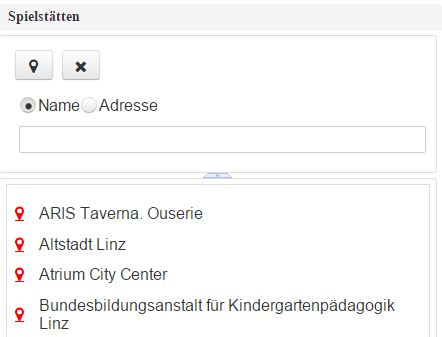
\includegraphics[scale=0.6]{\imagesRoot/web-view-venues.JPG}
	\caption
	{Übersicht Spielstätten}
\end{figure}
\ \newline
Es kann hier nachdem Namen und der Adresse gefiltert werden. Über einen Tooltip wird die Adresse der Spielstätte angezeigt. Über den Marker-Icon oder den Button mit den Marker-Icon kann der Dialog mit den Spielstättendetails geöffnet werden, wobei über den Marker-Icon nur die dazugehörige Spielstätten Details angezeigt werden und beim Button alle aktuell sichtbaren Spielstätten.
\newpage

\paragraph{Übersicht Aufführungen}
\ \newline 
Der Hauptteil der Seite sind die Aufführungen, die gruppiert nach deren Aufführungsdatum in einem Akkordion angezeigt werden. In der Tabelle werden nur die Aufführungszeiten angezeigt bei denen es mindestens eine Aufführung auf einer Spielstätte gibt. sollte dies nicht der Fall sein, so wird diese Spalte ausgeblendet.
\begin{figure}[h]
	\centering
	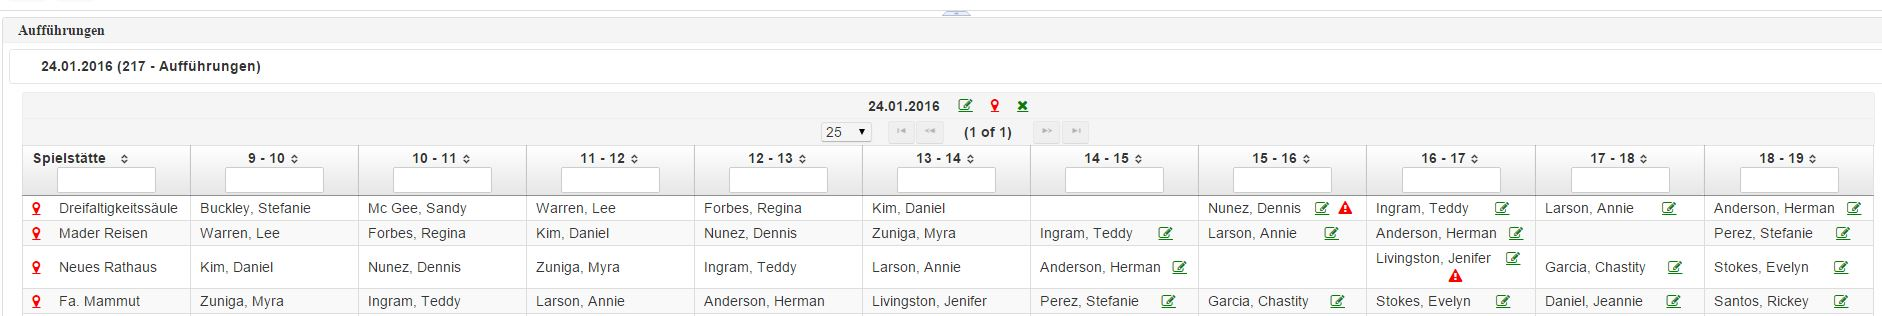
\includegraphics[scale=0.35]{\imagesRoot/web-view-performances.JPG}
	\caption
	{Übersicht Artisten}
\end{figure}
\ \newline
Die Aufführungen werden nach dem Spielstätten (Zeilen) und dessen Aufführungszeiten (Spalte) tabellarisch angezeigt. 
\newline
\newline
Folgende Aktionen stehen in dieser Ansicht für nicht eingeloggte Benutzer zur Verfügung.
\begin{enumerate}
	\item\emph{Dialog Artistendetails öffnen}
	\newline
	Durch das Klicken auf einen Artistennamen in einer Spalte öffnet sich der Dialog mit den Artistendetails
	\item\emph{Dialog einzelner Spielstättendetails öffnen}
	\newline
	Durch das Klicken auf einen Marker-Icon, der sich neben den Namen der Spielstätte befindet, öffnet sich ein Dialog mit den Spielstättendetails, wobei hier auch eine einfache Auflistung der Aufführungen an diesem Aufführungstag auf diese Spielstätte angeführt ist.
	\item\emph{Dialog aller Spielstättendetails öffnen}
	\newline
	Durch das Klicken auf einen Marker-Icon, der sich im Tabellenkopf befindet, öffnet sich ein Dialog mit den Spielstättendetails, wobei hier alle in der Tabelle befindlichen Spielstätten angezeigt werden so wie auch deren Aufführungen an diesem Aufführungstag.
\end{enumerate}
\ \newline
Folgende Aktionen stehen eingeloggten Benutzern zur Verfügung:
\begin{enumerate}
	\item\emph{Dialog zum Ändern einer/aller einzelnen der Aufführungen öffnen}
	\newline
	Durch das Klicken auf den Edit-Icon entweder neben dem Artistennamen einer Spalte oder dem Tabellenkopf kann ein Dialog geöffnet werden, über den die Aufführung geändert werden kann.
\end{enumerate}
\ \newline
Hierbei sei angemerkt das der Edit-Icon in den einzelnen Aufführungen nur ersichtlich wenn diese auch in der Zukunft liegen. Aufführungen die in der Vergangenheit liegen oder zu diesem Zeitpunkt stattfinden können nicht bearbeitet werden.
\newpage
Sollte ein Warn-Icon neben den Artistennamen einer Aufführung angezeigt werden, so wurde dieser verschoben, wobei die jeweils die Informationen der letzten Aufführungsdaten über einen Tooltip angezeigt werden.
\begin{figure}[h]
	\centering
	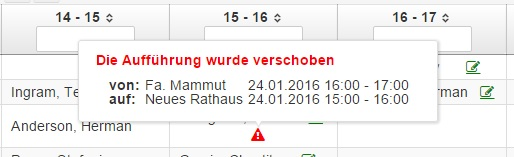
\includegraphics[scale=0.6]{\imagesRoot/web-view-performances-warn.JPG}
	\caption
	{Tooltip Warnung}
\end{figure}
\ \newline
Wenn man mit dem Cursor über einen Artistennamen in der Tabelle fährt, so wird ein Tooltip mit den wichtigsten Artistendetails angezeigt.
\begin{figure}[h]
	\centering
	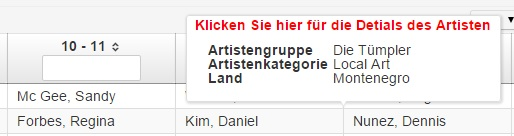
\includegraphics[scale=0.6]{\imagesRoot/web-view-performances-artist.JPG}
	\caption
	{Tooltip Artist}
\end{figure}
\ \newpage

\paragraph{Menü}
\ \newline 
Am unteren rechten Ende der Seite befindet sich ein sogenanntes Stack-Menu welches die Möglichkeit bietet, Aktionen auszuführen.
\newline
\newline
Sollte kein BenutzerIn eingeloggt sein, so sieht das Menü wie folgt aus.
\begin{figure}[h]
	\centering
	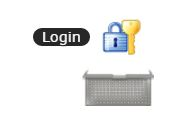
\includegraphics[scale=0.6]{\imagesRoot/web-view-stack-menu-not-logged.JPG}
	\caption
	{Stack Menü wenn nicht eingeloggt}
\end{figure}
\ \newline
Sollte ein BenutzerIn bereits eingeloggt sein, so sieht das Menü wie folgt aus.
\begin{figure}[h]
	\centering
	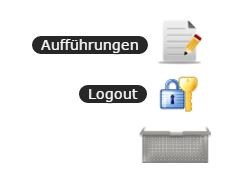
\includegraphics[scale=0.6]{\imagesRoot/web-view-stack-menu-logged.JPG}
	\caption
	{Stack Menü wenn eingeloggt}
\end{figure}
\ \newline
Durch Klicken auf den Korb kann das Menü auch weg geklappt werden.
\begin{figure}[h]
	\centering
	
\includegraphics[scale=0.6]{\imagesRoot/web-view-stack-menu-collapsed.JPG}
	\caption
	{Stack Menü zusammengeklappt}
\end{figure}
\ \newpage

\paragraph{Login}
\ \newline 
Für registrierte BenutzerInnen steht die Möglichkeit zur Verfügung  sich einzuloggen, damit diese BenutzerInnen Aufführungen anlegen und bestehende Aufführungen ändern können. Durch das Klicken auf das Login Menü wird ein Dialog geöffnet, über den man sich einloggen kann.
Durch Klicken auf das Loginmenü wird der Login Dialog geöffnet.
\begin{figure}[h]
	\centering
	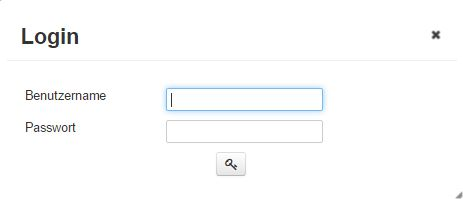
\includegraphics[scale=0.7]{\imagesRoot/web-view-dialog-login.JPG}
	\caption
	{Login Dialog}
\end{figure}
\ \newline
Sollten keine Daten eingegeben worden sein, so werden die Eingabefelder entsprechen markiert.
\begin{figure}[h]
	\centering
	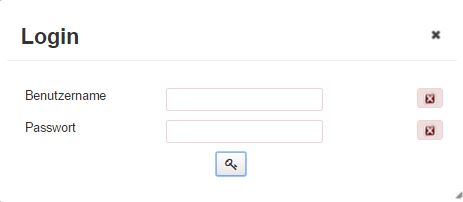
\includegraphics[scale=0.7]{\imagesRoot/web-view-dialog-login-invalid.JPG}
	\caption
	{Fehlerhafte Eingabe}
\end{figure}
\ \newline
Sollte der Login aufgrund fehlerhafter Login Daten fehlschlagen, so wird dies über eine Meldung angezeigt.
\begin{figure}[h]
	\centering
	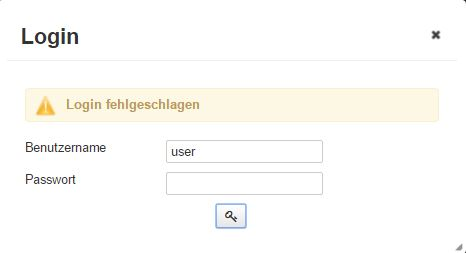
\includegraphics[scale=0.7]{\imagesRoot/web-view-dialog-login-failed.JPG}
	\caption
	{Login fehlgeschlagen}
\end{figure}
\ \newline
Nachdem einem erfolgreichen Login wird wieder auf die Hauptseite zurückgekehrt und der Dialog wird geschlossen. Anschließend stehen im Menü alle Funktionen für einen eingeloggten BenutzerIn zur Verfügung. Ebenso werden die Icons in der Aufführungstabelle angezeigt, über die der Aufführungsdialog angezeigt werden kann.
\newpage

\paragraph{Aufführung anlegen/bearbeiten}
\ \newline 
Über einen Dialog können bestehende Aufführungen bearbeitet sowie neue Aufführungen angelegt werden. Sollte der Dialog über den Edit-Icon in einer Spalte der Aufführungstabelle angelegt werden so wird diese Aufführung im Dialog gesetzt. Ansonsten wird ein leeres Formular angezeigt die AnwenderInnen können über eine Auswahl eine Aufführung auswählen. Diese Auswahl beschränkt sich auf die Aufführungen, die einerseits in der Seite zu sehen sind und andererseits auf die Aufführungen, die geändert werden dürfen.
\begin{figure}[h]
	\centering
	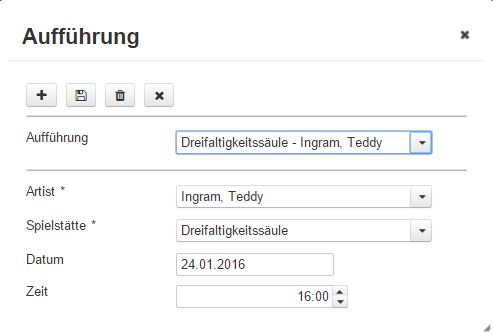
\includegraphics[scale=0.7]{\imagesRoot/web-view-dialog-performance.JPG}
	\caption
	{Dialog Aufführung anlegen/bearbeiten}
\end{figure}
\ \newline
Sollten die eingegebene Daten ungültig sein, so werden die Eingabefelder dementsprechend markiert.
\begin{figure}[h]
	\centering
	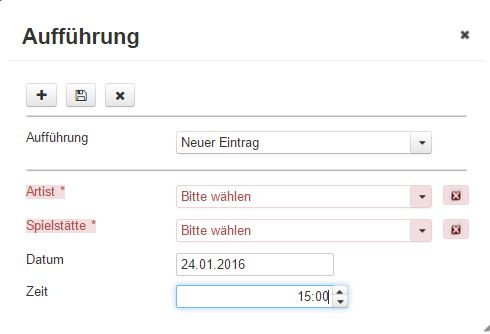
\includegraphics[scale=0.7]{\imagesRoot/web-view-dialog-performance-invalid.JPG}
	\caption
	{Ungültige Eingabe}
\end{figure}
\ \newpage
Sollte die Aufführung aufgrund eines logischen Fehlers fehlschlagen, so wird die eine entsprechende Meldung angezeigt.
\begin{figure}[h]
	\centering
	\includegraphics[scale=0.7]{\imagesRoot/web-view-dialog-performance-failed.JPG}
	\caption
	{Fehlgeschlagene logische Prüfung}
\end{figure}
\ \newpage

\paragraph{Dialog Spielstätte}
\ \newline 
Es können die Spielstätten in einem Dialog angezeigt werden wobei es hier zwei Möglichkeiten gibt:
\begin{enumerate}
	\item\emph{Mit Aufführungsdaten}
	\newline
	Sollte der Dialog über die Aufführungstabelle geöffnet werden, so sind hier die Aufführungsdetails der Spielstätte(n) am Aufführungstag angeführt. Durch das Öffnen des Dialogs über den Tabellenkopf werden alle Spielstätten dieser Tabelle angeführt, ansonsten nur eine einzeln. 
	\item\emph{Ohne Aufführungsdaten}
	\newline
	Sollte der Dialog über die Spielstättenauswahl geöffnet werden, so werden hier lediglich die Spielstättendaten angezeigt.
\end{enumerate}
\ \newline
Die Spielstätten werden hierbei auf einer Google-Maps angezeigt, wobei im Falle mit den Aufführungsdetails die einzelnen Spielstätten auch ausgewählt werden können und die dementsprechenden Ausführungsdetails ausgewählt werden.
\begin{figure}[h]
	\centering
	\includegraphics[scale=0.6]{\imagesRoot/web-view-dialog-venues-performances.JPG}
	\caption
	{Spielstätten Dialog mit Aufführungsdetails}
\end{figure}
\ \newline
Auch in dieser Tabelle werden über Tooltips Informationen des Artisten sowie auch von verschobenen Aufführungen angezeigt.
 \newpage
\begin{figure}[h]
	\centering
	\includegraphics[scale=0.6]{\imagesRoot/web-view-dialog-venues.JPG}
	\caption
	{Spielstätten Dialog ohne Aufführungsdetails}
\end{figure}
\end{document} 